 \documentclass[10pt, table, handout]{beamer}
\usetheme[progressbar=frametitle]{metropolis}
\usepackage{appendixnumberbeamer}
\usetikzlibrary{arrows.meta, positioning, quotes}
\usepackage[shortlabels]{enumitem}
\usepackage{xcolor}


\usepackage{booktabs}
\usepackage[scale=2]{ccicons}
\usepackage{ dsfont }

\usepackage{pgfplots}
\usepgfplotslibrary{dateplot}

\usepackage{xspace}
\newcommand{\themename}{\textbf{\textsc{metropolis}}\xspace}
\newcommand{\cb}{\cellcolor{blue!25}}


% Notation:
\newcommand{\cT}{\ensuremath{\mathcal{T}}}
\newcommand{\cD}{\ensuremath{\mathcal{D}}}
\newcommand{\cX}{\ensuremath{\mathcal{X}}}
\newcommand{\cY}{\ensuremath{\mathcal{Y}}}
\newcommand{\cZ}{\ensuremath{\mathcal{Z}}}
\newcommand{\cH}{\ensuremath{\mathcal{H}}}

\newcommand{\bR}{\ensuremath{\mathbb{R}}}
\newcommand{\bN}{\ensuremath{\mathbb{N}}}
\newcommand{\bP}{\ensuremath{\mathbb{P}}}


\title{Machine Learning I}
\subtitle{Lecture 18: Mathematical Foundations of Machine Learning}
% \date{\today}
\date{}
\author{Nathaniel Bade}
\institute{Northeastern University Department of Mathematics}
% \titlegraphic{\hfill\includegraphics[height=1.5cm]{logo.pdf}}

\begin{document}

\maketitle

\begin{frame}{Table of contents}
  \setbeamertemplate{section in toc}[sections numbered]
  \tableofcontents[hideallsubsections]
\end{frame}



\section{A Formal Model for Statistical Learning}


\begin{frame}[fragile]{Formal Model}
We will begin to construct a formal model for machine learning using the \textbf{partially approximately correct} model of Shalev-Shwartz and Ben-David. The text is highly encouraged, but I will include in the slides everything necessary for the homework. We will however strive to use the notation of Hastie, Tibshirani and Friedman.  

The goal of this lecture is to begin to provide a rigorous framework for statistical learning. We will first build our theory out in a rather simplified setting and then add layers of complexity. 

\end{frame}




\begin{frame}[fragile]{Formal Model: Example}
  \begin{minipage}[t][0.5\textheight][t]{\textwidth}
    \includegraphics[height=0.5\textheight]{L2MangoSpace.png}
        \centering
  \end{minipage}
  \vfill
  \begin{minipage}[t][0.5\textheight][t]{\textwidth}
In this lecture we will be considering supervised learning with a discrete label set. In supervised learning, a \textbf{learner} is an algorithm that will produce a function assigning a label to each element of some domain.\newline\pause

A guiding example: the perfect mango. 
  \end{minipage}

\end{frame}


\begin{frame}[fragile]{Formal Model: Example}
  \begin{minipage}[t][0.5\textheight][t]{\textwidth}
    \includegraphics[height=0.5\textheight]{L2MangoSpace.png}
        \centering
  \end{minipage}
  \vfill
  \begin{minipage}[t][0.5\textheight][t]{\textwidth}
Assume you have charted all the mangos you eat by color and hardness, recording which are perfectly ripe. A \textbf{learner} produce an algorithmic rule from this data set to label any mango as ripe or unripe.  
  \end{minipage}

\end{frame}






\begin{frame}[fragile]{Formal Model: Inputs and Outputs}
In the basic setting, the learner has access to the following:

\textbf{Learner Inputs:}
\begin{itemize}[label={}]
\item\textbf{Domain Set}: A set $\mathcal{X}$ providing a domain for the input $X$.\pause

\item\textbf{Label Set}: A (discrete) set $\mathcal{Y}$ providing the range for the output $Y$.\pause

\item\textbf{Training Data}: A sequence of $N$ pairs $\mathcal{T} = \{(x_1,y_1),\ldots,(x_N,y_N)\}$ in $\mathcal{X}\times \mathcal{Y}$.
\end{itemize}
 \pause

\textbf{Learner Output:}

\begin{itemize}
\item The \textbf{learners output} will be a \textbf{prediction rule} $h:\mathcal{X}\to \mathcal{Y}$. This function is also called a \textbf{predictor} or \textbf{classifier}. \pause\, We denote by $A(\mathcal{T}) = h_{\mathcal{T}}$ the \textbf{predictor} returned by an algorithm $A$ run on the training set $\mathcal{T}$.
\end{itemize}

\end{frame}



\begin{frame}[fragile]{Formal Model: Distribution Dependence}
  \begin{minipage}[t][0.5\textheight][t]{\textwidth}
    \includegraphics[height=0.5\textheight]{L2MangoSpace2.png}
        \centering
  \end{minipage}
  \vfill
  \begin{minipage}[t][0.5\textheight][t]{\textwidth}
\textbf{Data generation:} We assume that the mangos we have tasted are generated by a probability distribution $\mathcal{D}$ on $\mathcal{X}$. \pause

We also assume that there is a ``correct" labeling $f:\mathcal{X}\to\mathcal{Y}$. This will be relaxed shortly.\pause

For example, if $f(x)$ labels as ripe all points inside the central square, a change in distribution will changed the observed training data: \textbf{Uniform}
  \end{minipage}

\end{frame}




\begin{frame}[fragile]{Formal Model: Distribution Dependence}
  \begin{minipage}[t][0.5\textheight][t]{\textwidth}
    \includegraphics[height=0.5\textheight]{L2MangoSpace3.png}
        \centering
  \end{minipage}
  \vfill
  \begin{minipage}[t][0.5\textheight][t]{\textwidth}
\textbf{Data generation:} We assume that the mangos we have tasted are generated by a probability distribution $\mathcal{D}$ on $\mathcal{X}$. 

We also assume that there is a ``correct" labeling $f:\mathcal{X}\to\mathcal{Y}$. This will be relaxed shortly.

For example, if $f(x)$ labels as ripe all points inside the central square, a change in distribution will changed the observed training data: \textbf{Gaussian}
  \end{minipage}

\end{frame}




\begin{frame}[fragile]{Formal Model: Distribution Dependence}
  \begin{minipage}[t][0.5\textheight][t]{\textwidth}
    \includegraphics[height=0.5\textheight]{L2MangoSpace4.png}
        \centering
  \end{minipage}
  \vfill
  \begin{minipage}[t][0.5\textheight][t]{\textwidth}
\textbf{Data generation:} We assume that the mangos we have tasted are generated by a probability distribution $\mathcal{D}$ on $\mathcal{X}$. 

We also assume that there is a ``correct" labeling $f:\mathcal{X}\to\mathcal{Y}$. This will be relaxed shortly.

For example, if $f(x)$ labels as ripe all points inside the central square, a change in distribution will changed the observed training data: \textbf{Other}
  \end{minipage}

\end{frame}





\begin{frame}[fragile]{Empirical Risk Minimization}
Given a training set $\mathcal{T}$, a learner must return a reasonable classifier. Without access to the distribution $\mathcal{D}$ or the correct labeling $f$, the true error is not available. In the \textbf{Empirical risk minimization} framework we proceed by finding $h$ that minimizes a \textbf{loss function} $L$ on the training data. For example, for categorical data, we may minimize 1 - Accuracy: 

$$
L_{\mathcal{T}}(h) := \frac{\big| \{i: h(x_i)\neq y_i \} \big|}{N}\,.
$$
\pause
This loss called the \textbf{empirical error} or \textbf{empirical risk} since it is compute from the empirical data $\mathcal{T}$. \textbf{Empirical risk minimization} is the learning paradigm that states that this risk should be minimized. This is the main learning paradigm in this course (although we have seen others, like the perceptron algorithm and greedy algorithms like GD). 

\end{frame}


\begin{frame}[fragile]{Error}
The \textbf{true error of a classifier} $h$ is the probability $h$ does not predict the correct label for a point $x$ drawn from $\mathcal{X}$ according to the distribution $\mathcal{D}$:
\begin{flalign*}
\mathbf{Error:}\hspace{2em} L_{D,f}(h) := \mathbb{P}_{x\sim D}\big[ h(x) \neq f(x) \big]\,.&&
\end{flalign*}
It is also typical to use the distribution notation
\begin{flalign*}
\mathbf{Error:}\hspace{2em} L_{D,f}(h) := \mathcal{D}\big(\,\{x:h(x)\neq f(x)\}\big)\,.&&
\end{flalign*}
The error is the probability of randomly choosing an example $x$ for which $f(x)\neq h(x)$. 

This is also known as the \textbf{risk} or the \textbf{true error}.

\end{frame}



\begin{frame}[fragile]{Alternative Errors}
\textbf{Other notions of error:}  There are of course many notations of error, but accuracy 
$$
L_{D,f}(h) := \mathbb{P}_{x\sim D}\big[ h(x) \neq f(x) \big]
$$
is typically used for categorical variables. \newline

For quantitative variables, the usual error function is the RSS error
$$
\text{Err}_{\mathcal{T}} = E\big[ (h(x) - f(x))^2 \big]\,.
$$

\end{frame}




\begin{frame}[fragile]{Biased Empirical Risk Minimization}
The \textbf{empirical risk minimization} (\textbf{ERM}) rule tells us we should select a predictor $h$ that minimizes the training error
$$
L_{\mathcal{T}}(h)\,.
$$
However, if we let $h$ be an arbitrary function, we immediately overfit, since $h$ can take arbitrary values for each $x\in \mathcal{X}$.\pause A common solution is to apply \textbf{ERM} only over a restricted function space called a \textbf{hypothesis class}. \pause

For a hypothesis class $\mathcal{H}$, the \textbf{ERM}$_\mathcal{H}$ chooses a predictor from $\mathcal{H}$ with the lowest error over $\mathcal{T}$:
$$
\mathbf{ERM}_\mathcal{H}(\mathcal{T}) \in \text{argmin}_{h\in \mathcal{H}}\,L_{\mathcal{T}}(h)\,.
$$
Such a restriction is called an \textbf{inductive bias}.
\end{frame}




\begin{frame}[fragile]{Biased Empirical Risk Minimization}
We have seen many examples of hypothesis classes in this course:

\begin{itemize}
\item Linear separators and linear regressors.\pause
\item Polynomial separators and regressors with fixed degree. \pause
\item Radial basis kernels. \pause
\item Locally polynomial splines with fixed degree. \pause
\item Neural networks with fixed layer connects and layer sizes.\pause
\item Decision trees.\pause
\item Boosted models. \pause
\end{itemize}
Notice that many of these hypothesis classes fit in a larger hypothesis classes parameterized by their \textbf{hyperparmeters}. Hyperparameters are the parameters we do not allow to vary in the loss minimization framework. 
\end{frame}





\begin{frame}[fragile]{Biased Empirical Risk Minimization: Examples}
  \begin{minipage}[t][0.5\textheight][t]{\textwidth}
    \includegraphics[height=0.5\textheight]{L2Classifier.png}
        \centering
  \end{minipage}
  \vfill
  \begin{minipage}[t][0.5\textheight][t]{\textwidth}
The \textbf{indicator function} for any set $S\subseteq \mathcal{X}$ is
$$
\mathds{1}_S(x) = \begin{cases}
1&  x\in S
\\
0 & x\not\in S
\end{cases}\,,
$$
  \end{minipage}
\end{frame}



\begin{frame}[fragile]{Biased Empirical Risk Minimization: Examples}
  \begin{minipage}[t][0.5\textheight][t]{\textwidth}
    \includegraphics[height=0.5\textheight]{L2Classifier.png}
        \centering
  \end{minipage}
  \vfill
  \begin{minipage}[t][0.5\textheight][t]{\textwidth}
In the mango example, would could pick 
$$
\mathcal{H} = \{ \mathds{1}_{[a,b]\times[c,d]}\,|\, a,b,c,d\in [0,1]\}
$$ 
to be the set of indicator functions that is 1 on the interior of the square  $[a,b]\times[c,d]$ and 0 otherwise. We will see that restricting to this class \textit{cannot} overfit.
  \end{minipage}
\end{frame}




\begin{frame}[fragile]{Biased Empirical Risk Minimization: Examples}
  \begin{minipage}[t][0.5\textheight][t]{\textwidth}
    \includegraphics[height=0.5\textheight]{L2Classifier3.png}
        \centering
  \end{minipage}
  \vfill
  \begin{minipage}[t][0.5\textheight][t]{\textwidth}
Over the next few lectures, we're going to talk about how to use the ERM framework to prove statements about the accuracy of certain hypothesis classes. We will start small, talking about simple classifiers over known distributions, but at the end be able to make some very general statements about the learning power of classifiers like neural networks over unknown distributions. 
  \end{minipage}
\end{frame}


\section{Proving Bounds Using Realizability and I.I.D.}



\begin{frame}[fragile]{}
  \begin{minipage}[t][0.4\textheight][t]{\textwidth}
	\centering
	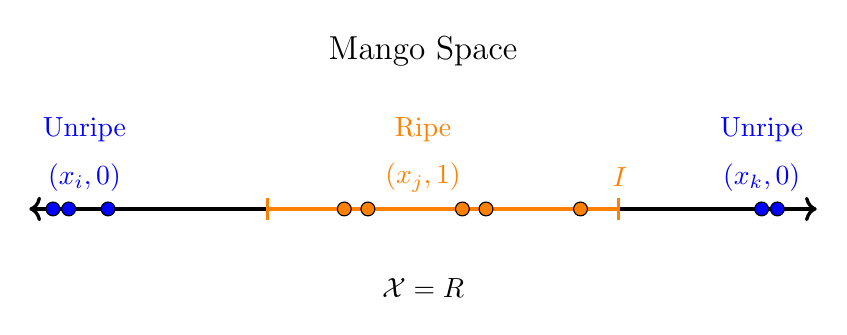
\begin{tikzpicture}
		\draw[<->,very thick] (-5,0) -- (5,0);
		\node at (0,2) {\large Mango Space} ;
		\node at (0,-1) {$\mathcal{X} = \mathbb{R}$} ;
		\node [color=blue] at (-4.3,1) {Unripe} ;
		\node [color=blue] at (4.3,1) {Unripe} ;
		\node [color=orange] at (0,1) {Ripe} ;
		\node [color=blue] at (-4.3,.4) {$(x_i,0)$} ;
		\node [color=blue] at (4.3,.4) {$(x_k,0)$} ;
		\node [color=orange] at (0,.4) {$(x_j,1)$} ;

		\draw[|-|,color=orange, very thick] (-2,0) -- (2.5,0);
		\node [color=orange] at (2.5,.4) {$I$} ;



		\node[circle,draw=black, fill=orange, inner sep=0pt,minimum size=5pt] at (2,0) {};
		\node[circle,draw=black, fill=orange, inner sep=0pt,minimum size=5pt] at (-1,0) {};
		\node[circle,draw=black, fill=orange, inner sep=0pt,minimum size=5pt] at (-.7,0) {};
		\node[circle,draw=black, fill=orange, inner sep=0pt,minimum size=5pt] at (.5,0) {};
		\node[circle,draw=black, fill=orange, inner sep=0pt,minimum size=5pt] at (.8,0) {};

		\node[circle,draw=black, fill=blue, inner sep=0pt,minimum size=5pt] at (-4.5,0) {};
		\node[circle,draw=black, fill=blue, inner sep=0pt,minimum size=5pt] at (-4,0) {};
		\node[circle,draw=black, fill=blue, inner sep=0pt,minimum size=5pt] at (-4.7,0) {};
		\node[circle,draw=black, fill=blue, inner sep=0pt,minimum size=5pt] at (4.3,0) {};
		\node[circle,draw=black, fill=blue, inner sep=0pt,minimum size=5pt] at (4.5,0) {};
	\end{tikzpicture}
  \end{minipage}
  \vfill
  \begin{minipage}[t][0.6\textheight][t]{\textwidth}
As a first example, we will compute the number of data points need to fit the 1D mango example. The input space will be $\mathcal{X} = \mathbb{R}$ and the label space will be $\mathcal{Y} = \{0,1\}$.\newline 

The hypothesis class is the class of indicator functions on intervals in $\mathbb{R}$ 
$$
\mathcal{H} = \{\mathds{1}_I\,:\,I = [a,b]\}\,.
$$\pause

The $\mathbf{ERM}_{\mathcal{H}}$ rule will be implemented by finding the smallest interval containing all data points labeled $1$. Above, $\mathbf{ERM}_{\mathcal{H}}(\mathcal{T}) = h_{\mathcal{T}}$.

\end{minipage}

\end{frame}








\begin{frame}[fragile]{}
  \begin{minipage}[t][0.4\textheight][t]{\textwidth}
	\centering
	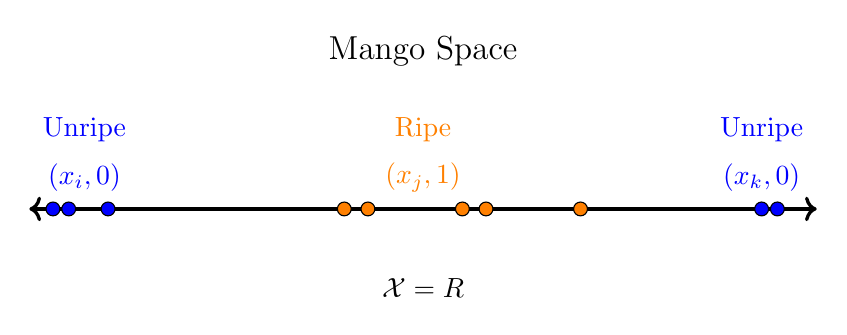
\begin{tikzpicture}
		\draw[<->,very thick] (-5,0) -- (5,0);
%		\draw[|-|,very thick] (-3,0) -- (4,0);
		\node at (0,2) {\large Mango Space} ;
		\node at (0,-1) {$\mathcal{X} = \mathbb{R}$} ;
		\node [color=blue] at (-4.3,1) {Unripe} ;
		\node [color=blue] at (4.3,1) {Unripe} ;
		\node [color=orange] at (0,1) {Ripe} ;
		\node [color=blue] at (-4.3,.4) {$(x_i,0)$} ;
		\node [color=blue] at (4.3,.4) {$(x_k,0)$} ;
		\node [color=orange] at (0,.4) {$(x_j,1)$} ;



		\node[circle,draw=black, fill=orange, inner sep=0pt,minimum size=5pt] at (2,0) {};
		\node[circle,draw=black, fill=orange, inner sep=0pt,minimum size=5pt] at (-1,0) {};
		\node[circle,draw=black, fill=orange, inner sep=0pt,minimum size=5pt] at (-.7,0) {};
		\node[circle,draw=black, fill=orange, inner sep=0pt,minimum size=5pt] at (.5,0) {};
		\node[circle,draw=black, fill=orange, inner sep=0pt,minimum size=5pt] at (.8,0) {};

		\node[circle,draw=black, fill=blue, inner sep=0pt,minimum size=5pt] at (-4.5,0) {};
		\node[circle,draw=black, fill=blue, inner sep=0pt,minimum size=5pt] at (-4,0) {};
		\node[circle,draw=black, fill=blue, inner sep=0pt,minimum size=5pt] at (-4.7,0) {};
		\node[circle,draw=black, fill=blue, inner sep=0pt,minimum size=5pt] at (4.3,0) {};
		\node[circle,draw=black, fill=blue, inner sep=0pt,minimum size=5pt] at (4.5,0) {};
	\end{tikzpicture}
  \end{minipage}
  \vfill
  \begin{minipage}[t][0.6\textheight][t]{\textwidth}

We will make two assumptions:\newline

\textbf{The I.I.D Assumption:} The examples in the training set $\mathcal{T}$ are independent and identically distributed (i.i.d.). That is, the probability the $i$'th point in the training set taking on a certain value depends only on $\mathcal{D}$.\newline \pause


\textbf{The Realizability Assumption:} The labels are actually generated by some $f\in \mathcal{H}$ and drawn from some distribution $\mathcal{D}$ on $\mathcal{X}$. 

  \end{minipage}

\end{frame}






\begin{frame}[fragile]{}
  \begin{minipage}[t][0.4\textheight][t]{\textwidth}
	\centering
	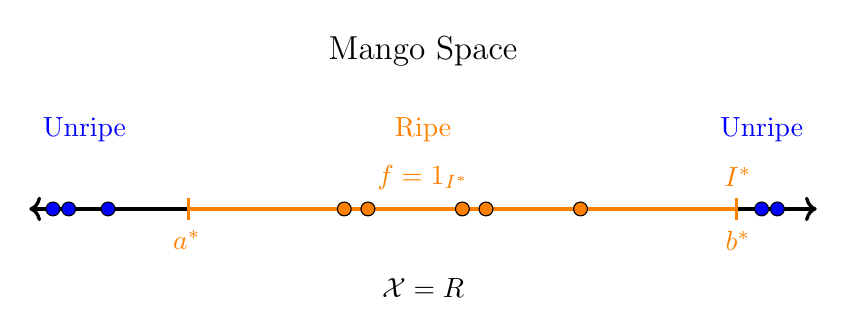
\begin{tikzpicture}
		\draw[<->,very thick] (-5,0) -- (5,0);
		\draw[color = orange, |-|,very thick] (-3,0) -- (4,0);
		\node[color=orange] at (4,.4) {$I^*$};
		\node at (0,2) {\large Mango Space} ;
		\node at (0,-1) {$\mathcal{X} = \mathbb{R}$} ;
		\node [color=blue] at (-4.3,1) {Unripe} ;
		\node [color=blue] at (4.3,1) {Unripe} ;
		\node [color=orange] at (0,1) {Ripe} ;

		\node [color=orange] at (0,.4) {$f = 1_{I^*}$} ;
		\node [color=orange] at (-3,-.4) {$a^*$} ;
		\node [color=orange] at (4,-.4) {$b^*$} ;



		\node[circle,draw=black, fill=orange, inner sep=0pt,minimum size=5pt] at (2,0) {};
		\node[circle,draw=black, fill=orange, inner sep=0pt,minimum size=5pt] at (-1,0) {};
		\node[circle,draw=black, fill=orange, inner sep=0pt,minimum size=5pt] at (-.7,0) {};
		\node[circle,draw=black, fill=orange, inner sep=0pt,minimum size=5pt] at (.5,0) {};
		\node[circle,draw=black, fill=orange, inner sep=0pt,minimum size=5pt] at (.8,0) {};

		\node[circle,draw=black, fill=blue, inner sep=0pt,minimum size=5pt] at (-4.5,0) {};
		\node[circle,draw=black, fill=blue, inner sep=0pt,minimum size=5pt] at (-4,0) {};
		\node[circle,draw=black, fill=blue, inner sep=0pt,minimum size=5pt] at (-4.7,0) {};
		\node[circle,draw=black, fill=blue, inner sep=0pt,minimum size=5pt] at (4.3,0) {};
		\node[circle,draw=black, fill=blue, inner sep=0pt,minimum size=5pt] at (4.5,0) {};
	\end{tikzpicture}
  \end{minipage}
  \vfill
  \begin{minipage}[t][0.6\textheight][t]{\textwidth}

We will make two assumptions:\newline

\textbf{The I.I.D Assumption:} The examples in the training set $\mathcal{T}$ are independent and identically distributed (i.i.d.). That is, the probability the $i$'th point in the training set taking on a certain value depends only on $\mathcal{D}$.\newline 


\textbf{The Realizability Assumption:} The labels are actually generated by some $f\in \mathcal{H}$ and drawn from some distribution $\mathcal{D}$ on $\mathcal{X}$. 
  \end{minipage}

\end{frame}





\begin{frame}[fragile]{}
  \begin{minipage}[t][0.4\textheight][t]{\textwidth}
	\centering
	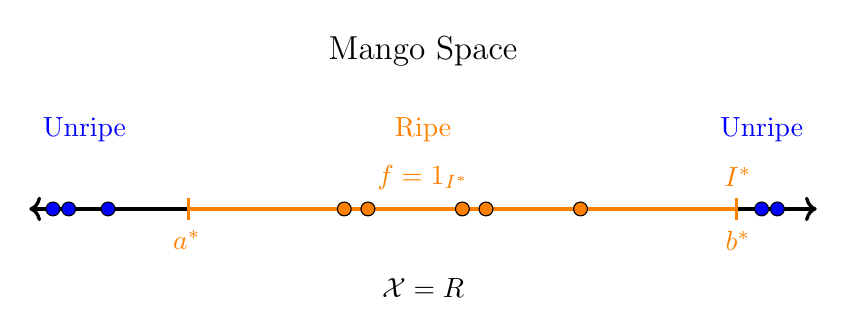
\begin{tikzpicture}
		\draw[<->,very thick] (-5,0) -- (5,0);
		\draw[color = orange, |-|,very thick] (-3,0) -- (4,0);
		\node[color=orange] at (4,.4) {$I^*$};
		\node at (0,2) {\large Mango Space} ;
		\node at (0,-1) {$\mathcal{X} = \mathbb{R}$} ;
		\node [color=blue] at (-4.3,1) {Unripe} ;
		\node [color=blue] at (4.3,1) {Unripe} ;
		\node [color=orange] at (0,1) {Ripe} ;

		\node [color=orange] at (0,.4) {$f = 1_{I^*}$} ;
		\node [color=orange] at (-3,-.4) {$a^*$} ;
		\node [color=orange] at (4,-.4) {$b^*$} ;



		\node[circle,draw=black, fill=orange, inner sep=0pt,minimum size=5pt] at (2,0) {};
		\node[circle,draw=black, fill=orange, inner sep=0pt,minimum size=5pt] at (-1,0) {};
		\node[circle,draw=black, fill=orange, inner sep=0pt,minimum size=5pt] at (-.7,0) {};
		\node[circle,draw=black, fill=orange, inner sep=0pt,minimum size=5pt] at (.5,0) {};
		\node[circle,draw=black, fill=orange, inner sep=0pt,minimum size=5pt] at (.8,0) {};

		\node[circle,draw=black, fill=blue, inner sep=0pt,minimum size=5pt] at (-4.5,0) {};
		\node[circle,draw=black, fill=blue, inner sep=0pt,minimum size=5pt] at (-4,0) {};
		\node[circle,draw=black, fill=blue, inner sep=0pt,minimum size=5pt] at (-4.7,0) {};
		\node[circle,draw=black, fill=blue, inner sep=0pt,minimum size=5pt] at (4.3,0) {};
		\node[circle,draw=black, fill=blue, inner sep=0pt,minimum size=5pt] at (4.5,0) {};
	\end{tikzpicture}
  \end{minipage}
  \vfill
  \begin{minipage}[t][0.6\textheight][t]{\textwidth}

\textbf{The Realizability Assumption:} The labels are actually generated by some $f\in \mathcal{H}$ and drawn from some distribution $\mathcal{D}$ on $\mathcal{X}$. \newline  

Realizability implies that for any training set $\mathcal{T}$, any ERM rule will return a classifier $h_{\mathcal{T}}$ with \textbf{training error} $L_{\mathcal{T}}(h_{\mathcal{T}})=0$.\newline \pause

But that does not meant that ERM returns $f$! We are not interested in \textbf{training error}, we are interested in the \textbf{true error} $L_{(f,\mathcal{D})}(h_{\mathcal{T}})$.
  \end{minipage}

\end{frame}







\begin{frame}[fragile]{}
  \begin{minipage}[t][0.4\textheight][t]{\textwidth}
	\centering
	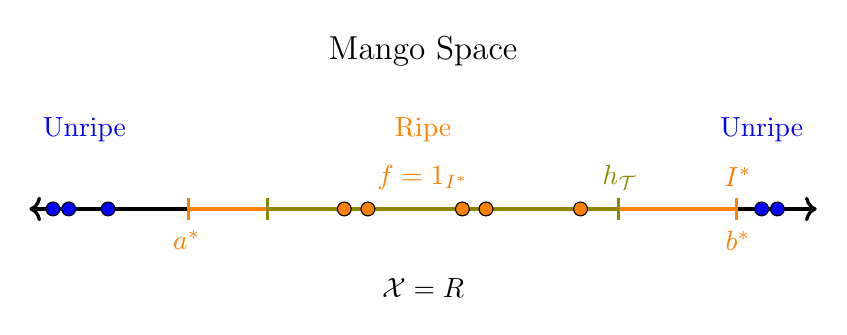
\begin{tikzpicture}
		\draw[<->,very thick] (-5,0) -- (5,0);
		\draw[color = orange, |-|,very thick] (-3,0) -- (4,0);
		\node[color=orange] at (4,.4) {$I^*$};
		\node at (0,2) {\large Mango Space} ;
		\node at (0,-1) {$\mathcal{X} = \mathbb{R}$} ;
		\node [color=blue] at (-4.3,1) {Unripe} ;
		\node [color=blue] at (4.3,1) {Unripe} ;
		\node [color=orange] at (0,1) {Ripe} ;

		\node [color=orange] at (0,.4) {$f = 1_{I^*}$} ;
		\node [color=orange] at (-3,-.4) {$a^*$} ;
		\node [color=orange] at (4,-.4) {$b^*$} ;

		\draw [color=olive, |-|,very thick] (-2,0) -- (2.5,0);
		\node [color=olive] at (2.5,.4) {$h_{\mathcal{T}}$} ;



		\node[circle,draw=black, fill=orange, inner sep=0pt,minimum size=5pt] at (2,0) {};
		\node[circle,draw=black, fill=orange, inner sep=0pt,minimum size=5pt] at (-1,0) {};
		\node[circle,draw=black, fill=orange, inner sep=0pt,minimum size=5pt] at (-.7,0) {};
		\node[circle,draw=black, fill=orange, inner sep=0pt,minimum size=5pt] at (.5,0) {};
		\node[circle,draw=black, fill=orange, inner sep=0pt,minimum size=5pt] at (.8,0) {};

		\node[circle,draw=black, fill=blue, inner sep=0pt,minimum size=5pt] at (-4.5,0) {};
		\node[circle,draw=black, fill=blue, inner sep=0pt,minimum size=5pt] at (-4,0) {};
		\node[circle,draw=black, fill=blue, inner sep=0pt,minimum size=5pt] at (-4.7,0) {};
		\node[circle,draw=black, fill=blue, inner sep=0pt,minimum size=5pt] at (4.3,0) {};
		\node[circle,draw=black, fill=blue, inner sep=0pt,minimum size=5pt] at (4.5,0) {};
	\end{tikzpicture}
  \end{minipage}
  \vfill
  \begin{minipage}[t][0.6\textheight][t]{\textwidth}

\textbf{The Realizability Assumption:} The data is actually generated by some $f\in \mathcal{H}$ and some distribution $\mathcal{D}$ on $\mathcal{X}$.\newline  

Realizability implies that for any training set $\mathcal{T}$, any ERM rule will return a classifier $h_{\mathcal{T}}$ with \textbf{training error} $L_{\mathcal{T}}(h_{\mathcal{T}})=0$.\newline

But that does not meant that ERM returns $f$! We are not interested in \textbf{training error}, we are interested in the \textbf{true error} $L_{(f,\mathcal{D})}(h_{\mathcal{T}})$.
  \end{minipage}

\end{frame}






\begin{frame}[fragile]{}
  \begin{minipage}[t][0.4\textheight][t]{\textwidth}
	\centering
	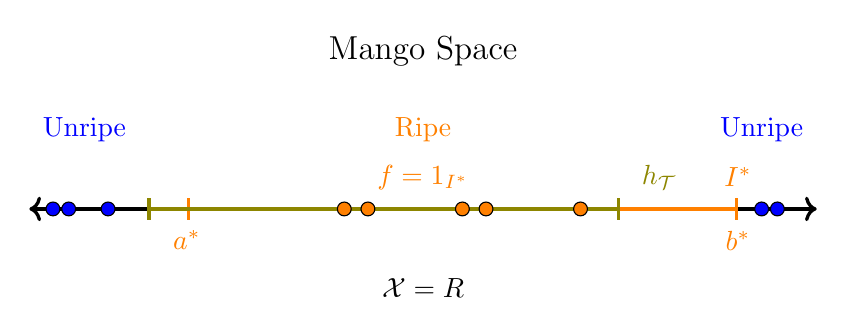
\begin{tikzpicture}
		\draw[<->,very thick] (-5,0) -- (5,0);
		\draw[color = orange, |-|,very thick] (-3,0) -- (4,0);
		\node[color=orange] at (4,.4) {$I^*$};
		\node at (0,2) {\large Mango Space} ;
		\node at (0,-1) {$\mathcal{X} = \mathbb{R}$} ;
		\node [color=blue] at (-4.3,1) {Unripe} ;
		\node [color=blue] at (4.3,1) {Unripe} ;
		\node [color=orange] at (0,1) {Ripe} ;

		\node [color=orange] at (0,.4) {$f = 1_{I^*}$} ;
		\node [color=orange] at (-3,-.4) {$a^*$} ;
		\node [color=orange] at (4,-.4) {$b^*$} ;

		\draw [color=olive, |-|,very thick] (-3.5,0) -- (2.5,0);
		\node [color=olive] at (3,.4) {$h_{\mathcal{T}}$} ;



		\node[circle,draw=black, fill=orange, inner sep=0pt,minimum size=5pt] at (2,0) {};
		\node[circle,draw=black, fill=orange, inner sep=0pt,minimum size=5pt] at (-1,0) {};
		\node[circle,draw=black, fill=orange, inner sep=0pt,minimum size=5pt] at (-.7,0) {};
		\node[circle,draw=black, fill=orange, inner sep=0pt,minimum size=5pt] at (.5,0) {};
		\node[circle,draw=black, fill=orange, inner sep=0pt,minimum size=5pt] at (.8,0) {};

		\node[circle,draw=black, fill=blue, inner sep=0pt,minimum size=5pt] at (-4.5,0) {};
		\node[circle,draw=black, fill=blue, inner sep=0pt,minimum size=5pt] at (-4,0) {};
		\node[circle,draw=black, fill=blue, inner sep=0pt,minimum size=5pt] at (-4.7,0) {};
		\node[circle,draw=black, fill=blue, inner sep=0pt,minimum size=5pt] at (4.3,0) {};
		\node[circle,draw=black, fill=blue, inner sep=0pt,minimum size=5pt] at (4.5,0) {};
	\end{tikzpicture}
  \end{minipage}
  \vfill
  \begin{minipage}[t][0.6\textheight][t]{\textwidth}

\textbf{The Realizability Assumption:} The data is actually generated by some $f\in \mathcal{H}$ and some distribution $\mathcal{D}$ on $\mathcal{X}$.\newline  

Realizability implies that for any training set $\mathcal{T}$, any ERM rule will return a classifier $h_{\mathcal{T}}$ with \textbf{training error} $L_{\mathcal{T}}(h_{\mathcal{T}})=0$.\newline

But that does not meant that ERM returns $f$! We are not interested in \textbf{training error}, we are interested in the \textbf{true error} $L_{(f,\mathcal{D})}(h_{\mathcal{T}})$.
  \end{minipage}

\end{frame}





\begin{frame}[fragile]{}
  \begin{minipage}[t][0.4\textheight][t]{\textwidth}
	\centering
	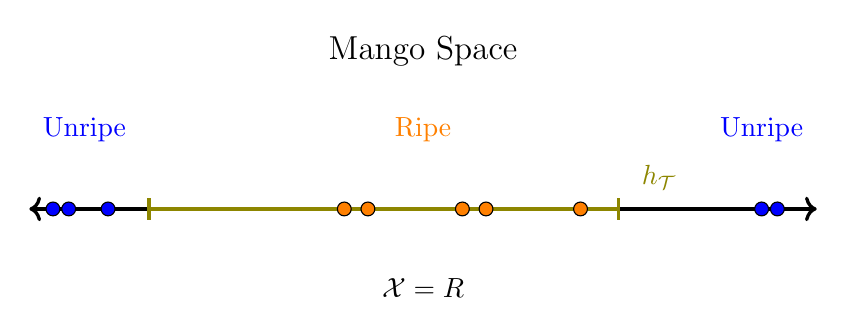
\begin{tikzpicture}
		\draw[<->,very thick] (-5,0) -- (5,0);
		\node at (0,2) {\large Mango Space} ;
		\node at (0,-1) {$\mathcal{X} = \mathbb{R}$} ;
		\node [color=blue] at (-4.3,1) {Unripe} ;
		\node [color=blue] at (4.3,1) {Unripe} ;
		\node [color=orange] at (0,1) {Ripe} ;

		\draw [color=olive, |-|,very thick] (-3.5,0) -- (2.5,0);
		\node [color=olive] at (3,.4) {$h_{\mathcal{T}}$} ;



		\node[circle,draw=black, fill=orange, inner sep=0pt,minimum size=5pt] at (2,0) {};
		\node[circle,draw=black, fill=orange, inner sep=0pt,minimum size=5pt] at (-1,0) {};
		\node[circle,draw=black, fill=orange, inner sep=0pt,minimum size=5pt] at (-.7,0) {};
		\node[circle,draw=black, fill=orange, inner sep=0pt,minimum size=5pt] at (.5,0) {};
		\node[circle,draw=black, fill=orange, inner sep=0pt,minimum size=5pt] at (.8,0) {};

		\node[circle,draw=black, fill=blue, inner sep=0pt,minimum size=5pt] at (-4.5,0) {};
		\node[circle,draw=black, fill=blue, inner sep=0pt,minimum size=5pt] at (-4,0) {};
		\node[circle,draw=black, fill=blue, inner sep=0pt,minimum size=5pt] at (-4.7,0) {};
		\node[circle,draw=black, fill=blue, inner sep=0pt,minimum size=5pt] at (4.3,0) {};
		\node[circle,draw=black, fill=blue, inner sep=0pt,minimum size=5pt] at (4.5,0) {};
	\end{tikzpicture}
  \end{minipage}
  \vfill
  \begin{minipage}[t][0.6\textheight][t]{\textwidth}

\textbf{The Realizability Assumption:} The data is actually generated by some $f\in \mathcal{H}$ and some distribution $\mathcal{D}$ on $\mathcal{X}$.\newline  

Realizability implies that for any training set $\mathcal{T}$, any ERM rule will return a classifier $h_{\mathcal{T}}$ with \textbf{training error} $L_{\mathcal{T}}(h_{\mathcal{T}})=0$.\newline

But that does not meant that ERM returns $f$! We are not interested in \textbf{training error}, we are interested in the \textbf{true error} $L_{(f,\mathcal{D})}(h_{\mathcal{T}})$.
  \end{minipage}

\end{frame}








\begin{frame}[fragile]{}
  \begin{minipage}[t][0.4\textheight][t]{\textwidth}
	\centering
	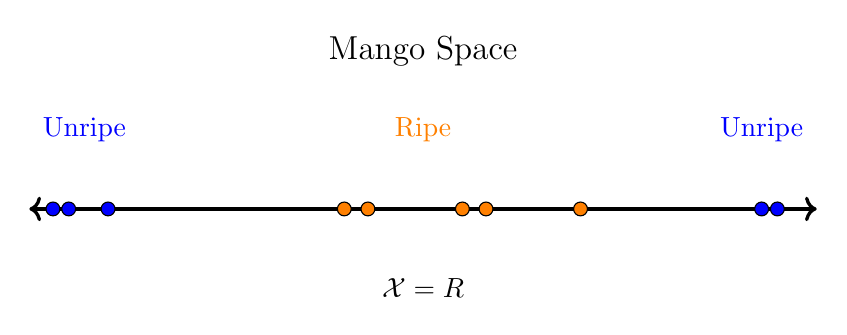
\begin{tikzpicture}
		\draw[<->,very thick] (-5,0) -- (5,0);
		\node at (0,2) {\large Mango Space} ;
		\node at (0,-1) {$\mathcal{X} = \mathbb{R}$} ;
		\node [color=blue] at (-4.3,1) {Unripe} ;
		\node [color=blue] at (4.3,1) {Unripe} ;
		\node [color=orange] at (0,1) {Ripe} ;



		\node[circle,draw=black, fill=orange, inner sep=0pt,minimum size=5pt] at (2,0) {};
		\node[circle,draw=black, fill=orange, inner sep=0pt,minimum size=5pt] at (-1,0) {};
		\node[circle,draw=black, fill=orange, inner sep=0pt,minimum size=5pt] at (-.7,0) {};
		\node[circle,draw=black, fill=orange, inner sep=0pt,minimum size=5pt] at (.5,0) {};
		\node[circle,draw=black, fill=orange, inner sep=0pt,minimum size=5pt] at (.8,0) {};

		\node[circle,draw=black, fill=blue, inner sep=0pt,minimum size=5pt] at (-4.5,0) {};
		\node[circle,draw=black, fill=blue, inner sep=0pt,minimum size=5pt] at (-4,0) {};
		\node[circle,draw=black, fill=blue, inner sep=0pt,minimum size=5pt] at (-4.7,0) {};
		\node[circle,draw=black, fill=blue, inner sep=0pt,minimum size=5pt] at (4.3,0) {};
		\node[circle,draw=black, fill=blue, inner sep=0pt,minimum size=5pt] at (4.5,0) {};
	\end{tikzpicture}
  \end{minipage}
  \vfill
  \begin{minipage}[t][0.6\textheight][t]{\textwidth}

Let $\epsilon\in (0,1)$ be the \textbf{target accuracy}, that is we interpret the event $L_{(\mathcal{D},f)}(h_{\mathcal{T}})>\epsilon$ as a \textbf{failure} of the learning algorithm. \newline\pause

We want to derive an upper bound for the probability $\delta$ of picking a \textbf{non representative training set}, that is a training set $\mathcal{T}$ with $N$ elements such that $L_{(\mathcal{D},f)}(h_{\mathcal{T}})>\epsilon$. We call $(1-\delta)$ the \textbf{confidence parameter}. 

 \end{minipage}

\end{frame}











\begin{frame}[fragile]{}

The goal is to find an upper bound for the probability of a picking a training set $\mathcal{T}\in \mathcal{D}^N$ that yields to classifier $h$ whose true error is larger than $\epsilon$:
$$
\delta = \mathcal{D}^N\big(\{\mathcal{T}\,:\, L_{(\mathcal{D},f)}(h_{\mathcal{T}}) > \epsilon\,\}\big)\,.
$$\pause

We will proceed in two steps:
\begin{itemize}
\item Step 1: Find a partition of the training sets $M\subset \mathcal{D}^N$ that guarantees that if $L_{(\mathcal{D},f)}(h_{\mathcal{T}}) < \epsilon$ then $\mathcal{T}\in M$.

\item Step 2: Derive an upper bound on the probability that $\mathcal{T}\not\in M$.
\end{itemize}

This upper bound will then give an upper bound for $\delta$. 

\end{frame}








\begin{frame}[fragile]{}
  \begin{minipage}[t][0.4\textheight][t]{\textwidth}
	\centering
	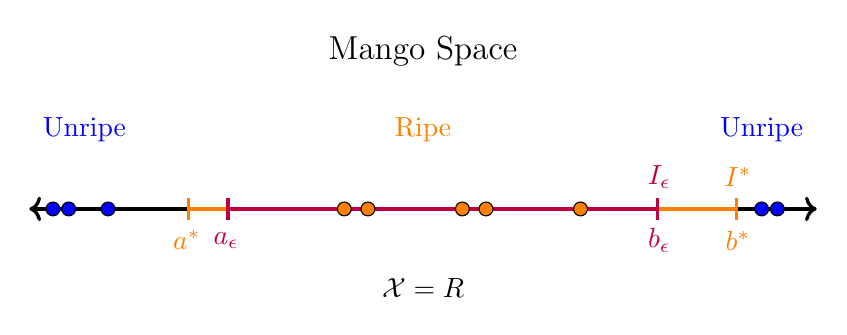
\begin{tikzpicture}
		\draw[<->,very thick] (-5,0) -- (5,0);
		\draw[color = orange, |-|,very thick] (-3,0) -- (4,0);
		\node[color=orange] at (4,.4) {$I^*$};
		\node at (0,2) {\large Mango Space} ;
		\node at (0,-1) {$\mathcal{X} = \mathbb{R}$} ;
		\node [color=blue] at (-4.3,1) {Unripe} ;
		\node [color=blue] at (4.3,1) {Unripe} ;
		\node [color=orange] at (0,1) {Ripe} ;

		\node [color=orange] at (-3,-.4) {$a^*$} ;
		\node [color=orange] at (4,-.4) {$b^*$} ;

		\draw [color=purple, |-|,very thick] (-2.5,0) -- (3,0);
		\node [color=purple] at (3,.4) {$I_\epsilon$} ;
		\node [color=purple] at (-2.5,-.4) {$a_\epsilon$} ;
		\node [color=purple] at (3,-.4) {$b_\epsilon$} ;

%		\draw [color=olive, |-|,very thick] (-3.5,0) -- (2.5,0);
%		\node [color=olive] at (3,.4) {$h_{\mathcal{T}}$} ;



		\node[circle,draw=black, fill=orange, inner sep=0pt,minimum size=5pt] at (2,0) {};
		\node[circle,draw=black, fill=orange, inner sep=0pt,minimum size=5pt] at (-1,0) {};
		\node[circle,draw=black, fill=orange, inner sep=0pt,minimum size=5pt] at (-.7,0) {};
		\node[circle,draw=black, fill=orange, inner sep=0pt,minimum size=5pt] at (.5,0) {};
		\node[circle,draw=black, fill=orange, inner sep=0pt,minimum size=5pt] at (.8,0) {};

		\node[circle,draw=black, fill=blue, inner sep=0pt,minimum size=5pt] at (-4.5,0) {};
		\node[circle,draw=black, fill=blue, inner sep=0pt,minimum size=5pt] at (-4,0) {};
		\node[circle,draw=black, fill=blue, inner sep=0pt,minimum size=5pt] at (-4.7,0) {};
		\node[circle,draw=black, fill=blue, inner sep=0pt,minimum size=5pt] at (4.3,0) {};
		\node[circle,draw=black, fill=blue, inner sep=0pt,minimum size=5pt] at (4.5,0) {};
	\end{tikzpicture}
  \end{minipage}
  \vfill
  \begin{minipage}[t][0.6\textheight][t]{\textwidth}
  	Let $I^* = [a^*,b^*]$ be the actual interval of ripeness. Pick $I_{\epsilon}=[a_\epsilon,b_\epsilon] \subset I^*$ so that both $\mathcal{D}([a^*,a_{\epsilon}]) = \epsilon/2$ and $\mathcal{D}([b_\epsilon, b^*]) = \epsilon/2$.\newline\pause

This means that the region $I^*-I_\epsilon$ contains less than $\epsilon$ of the total probability, ie $\mathcal{D}(I^*-I_\epsilon)=\epsilon$.\newline\pause

Then, if there exists $x_i, x_j\in\mathcal{T}$ such that $x_i\in [a_*, a_\epsilon]$ and $x_j\in [b_\epsilon, b_*]$, the ERM rule returns a classifier with error at most $\epsilon$. 

  \end{minipage}

\end{frame}







\begin{frame}[fragile]{}
  \begin{minipage}[t][0.4\textheight][t]{\textwidth}
	\centering
	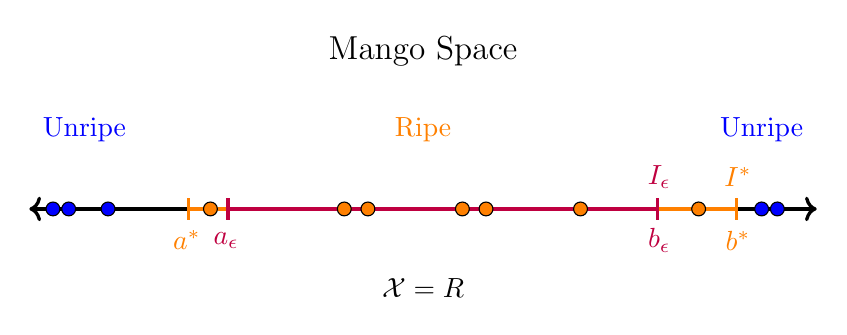
\begin{tikzpicture}
		\draw[<->,very thick] (-5,0) -- (5,0);
		\draw[color = orange, |-|,very thick] (-3,0) -- (4,0);
		\node[color=orange] at (4,.4) {$I^*$};
		\node at (0,2) {\large Mango Space} ;
		\node at (0,-1) {$\mathcal{X} = \mathbb{R}$} ;
		\node [color=blue] at (-4.3,1) {Unripe} ;
		\node [color=blue] at (4.3,1) {Unripe} ;
		\node [color=orange] at (0,1) {Ripe} ;

		\node [color=orange] at (-3,-.4) {$a^*$} ;
		\node [color=orange] at (4,-.4) {$b^*$} ;

		\draw [color=purple, |-|,very thick] (-2.5,0) -- (3,0);
		\node [color=purple] at (3,.4) {$I_\epsilon$} ;
		\node [color=purple] at (-2.5,-.4) {$a_\epsilon$} ;
		\node [color=purple] at (3,-.4) {$b_\epsilon$} ;

%		\draw [color=olive, |-|,very thick] (-3.5,0) -- (2.5,0);
%		\node [color=olive] at (3,.4) {$h_{\mathcal{T}}$} ;



		\node[circle,draw=black, fill=orange, inner sep=0pt,minimum size=5pt] at (2,0) {};
		\node[circle,draw=black, fill=orange, inner sep=0pt,minimum size=5pt] at (-1,0) {};
		\node[circle,draw=black, fill=orange, inner sep=0pt,minimum size=5pt] at (-.7,0) {};
		\node[circle,draw=black, fill=orange, inner sep=0pt,minimum size=5pt] at (.5,0) {};
		\node[circle,draw=black, fill=orange, inner sep=0pt,minimum size=5pt] at (.8,0) {};
		\node[circle,draw=black, fill=orange, inner sep=0pt,minimum size=5pt] at (-2.7,0) {};
		\node[circle,draw=black, fill=orange, inner sep=0pt,minimum size=5pt] at (3.5,0) {};

		\node[circle,draw=black, fill=blue, inner sep=0pt,minimum size=5pt] at (-4.5,0) {};
		\node[circle,draw=black, fill=blue, inner sep=0pt,minimum size=5pt] at (-4,0) {};
		\node[circle,draw=black, fill=blue, inner sep=0pt,minimum size=5pt] at (-4.7,0) {};
		\node[circle,draw=black, fill=blue, inner sep=0pt,minimum size=5pt] at (4.3,0) {};
		\node[circle,draw=black, fill=blue, inner sep=0pt,minimum size=5pt] at (4.5,0) {};
	\end{tikzpicture}
  \end{minipage}
  \vfill
  \begin{minipage}[t][0.6\textheight][t]{\textwidth}
	Let $I^* = [a^*,b^*]$ be the actual interval of ripeness. Pick $I_{\epsilon}=[a_\epsilon,b_\epsilon] \subset I^*$ so that both $\mathcal{D}([a^*,a_{\epsilon}]) = \epsilon/2$ and $\mathcal{D}([b_\epsilon, b^*]) = \epsilon/2$.\newline

This means that the region $I^*-I_\epsilon$ contains less than $\epsilon$ of the total probability, ie $\mathcal{D}(I^*-I_\epsilon)=\epsilon$.\newline

Then, if there exists $x_i, x_j\in\mathcal{T}$ such that $x_i\in [a_*, a_\epsilon]$ and $x_j\in [b_\epsilon, b_*]$, the ERM rule returns a classifier with error at most $\epsilon$. 

  \end{minipage}

\end{frame}






\begin{frame}[fragile]{}
  \begin{minipage}[t][0.4\textheight][t]{\textwidth}
	\centering
	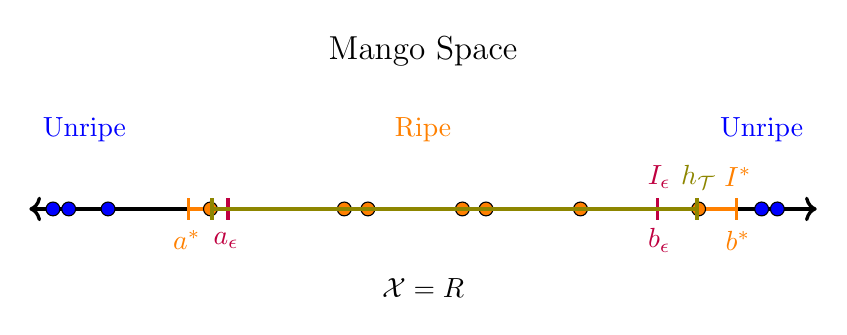
\begin{tikzpicture}
		\draw[<->,very thick] (-5,0) -- (5,0);
		\draw[color = orange, |-|,very thick] (-3,0) -- (4,0);
		\node[color=orange] at (4,.4) {$I^*$};
		\node at (0,2) {\large Mango Space} ;
		\node at (0,-1) {$\mathcal{X} = \mathbb{R}$} ;
		\node [color=blue] at (-4.3,1) {Unripe} ;
		\node [color=blue] at (4.3,1) {Unripe} ;
		\node [color=orange] at (0,1) {Ripe} ;

		\node [color=orange] at (-3,-.4) {$a^*$} ;
		\node [color=orange] at (4,-.4) {$b^*$} ;

		\draw [color=purple, |-|,very thick] (-2.5,0) -- (3,0);
		\node [color=purple] at (3,.4) {$I_\epsilon$} ;
		\node [color=purple] at (-2.5,-.4) {$a_\epsilon$} ;
		\node [color=purple] at (3,-.4) {$b_\epsilon$} ;



		\node[circle,draw=black, fill=orange, inner sep=0pt,minimum size=5pt] at (2,0) {};
		\node[circle,draw=black, fill=orange, inner sep=0pt,minimum size=5pt] at (-1,0) {};
		\node[circle,draw=black, fill=orange, inner sep=0pt,minimum size=5pt] at (-.7,0) {};
		\node[circle,draw=black, fill=orange, inner sep=0pt,minimum size=5pt] at (.5,0) {};
		\node[circle,draw=black, fill=orange, inner sep=0pt,minimum size=5pt] at (.8,0) {};
		\node[circle,draw=black, fill=orange, inner sep=0pt,minimum size=5pt] at (-2.7,0) {};
		\node[circle,draw=black, fill=orange, inner sep=0pt,minimum size=5pt] at (3.5,0) {};

		\node[circle,draw=black, fill=blue, inner sep=0pt,minimum size=5pt] at (-4.5,0) {};
		\node[circle,draw=black, fill=blue, inner sep=0pt,minimum size=5pt] at (-4,0) {};
		\node[circle,draw=black, fill=blue, inner sep=0pt,minimum size=5pt] at (-4.7,0) {};
		\node[circle,draw=black, fill=blue, inner sep=0pt,minimum size=5pt] at (4.3,0) {};
		\node[circle,draw=black, fill=blue, inner sep=0pt,minimum size=5pt] at (4.5,0) {};

		\draw [color=olive, |-|,very thick] (-2.7,0) -- (3.5,0);
   		\node [color=olive] at (3.5,.4) {$h_{\mathcal{T}}$} ;
	\end{tikzpicture}
  \end{minipage}
  \vfill
  \begin{minipage}[t][0.6\textheight][t]{\textwidth}
	Let $I^* = [a^*,b^*]$ be the actual interval of ripeness. Pick $I_{\epsilon}=[a_\epsilon,b_\epsilon] \subset I^*$ so that both $\mathcal{D}([a^*,a_{\epsilon}]) = \epsilon/2$ and $\mathcal{D}([b_\epsilon, b^*]) = \epsilon/2$.\newline

This means that the region $I^*-I_\epsilon$ contains less than $\epsilon$ of the total probability, ie $\mathcal{D}(I^*-I_\epsilon)=\epsilon$.\newline

Then, if there exists $x_i, x_j\in\mathcal{T}$ such that $x_i\in [a_*, a_\epsilon]$ and $x_j\in [b_\epsilon, b_*]$, the ERM rule returns a classifier with error at most $\epsilon$. 

  \end{minipage}

\end{frame}




\begin{frame}[fragile]{}
  \begin{minipage}[t][0.4\textheight][t]{\textwidth}
	\centering
	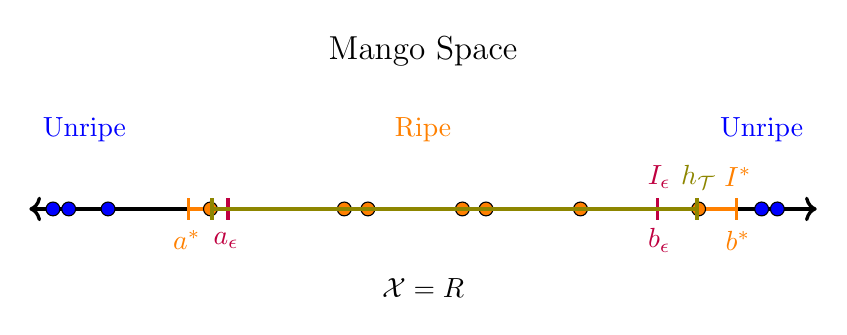
\begin{tikzpicture}
		\draw[<->,very thick] (-5,0) -- (5,0);
		\draw[color = orange, |-|,very thick] (-3,0) -- (4,0);
		\node[color=orange] at (4,.4) {$I^*$};
		\node at (0,2) {\large Mango Space} ;
		\node at (0,-1) {$\mathcal{X} = \mathbb{R}$} ;
		\node [color=blue] at (-4.3,1) {Unripe} ;
		\node [color=blue] at (4.3,1) {Unripe} ;
		\node [color=orange] at (0,1) {Ripe} ;

		\node [color=orange] at (-3,-.4) {$a^*$} ;
		\node [color=orange] at (4,-.4) {$b^*$} ;

		\draw [color=purple, |-|,very thick] (-2.5,0) -- (3,0);
		\node [color=purple] at (3,.4) {$I_\epsilon$} ;
		\node [color=purple] at (-2.5,-.4) {$a_\epsilon$} ;
		\node [color=purple] at (3,-.4) {$b_\epsilon$} ;



		\node[circle,draw=black, fill=orange, inner sep=0pt,minimum size=5pt] at (2,0) {};
		\node[circle,draw=black, fill=orange, inner sep=0pt,minimum size=5pt] at (-1,0) {};
		\node[circle,draw=black, fill=orange, inner sep=0pt,minimum size=5pt] at (-.7,0) {};
		\node[circle,draw=black, fill=orange, inner sep=0pt,minimum size=5pt] at (.5,0) {};
		\node[circle,draw=black, fill=orange, inner sep=0pt,minimum size=5pt] at (.8,0) {};
		\node[circle,draw=black, fill=orange, inner sep=0pt,minimum size=5pt] at (-2.7,0) {};
		\node[circle,draw=black, fill=orange, inner sep=0pt,minimum size=5pt] at (3.5,0) {};

		\node[circle,draw=black, fill=blue, inner sep=0pt,minimum size=5pt] at (-4.5,0) {};
		\node[circle,draw=black, fill=blue, inner sep=0pt,minimum size=5pt] at (-4,0) {};
		\node[circle,draw=black, fill=blue, inner sep=0pt,minimum size=5pt] at (-4.7,0) {};
		\node[circle,draw=black, fill=blue, inner sep=0pt,minimum size=5pt] at (4.3,0) {};
		\node[circle,draw=black, fill=blue, inner sep=0pt,minimum size=5pt] at (4.5,0) {};

		\draw [color=olive, |-|,very thick] (-2.7,0) -- (3.5,0);
   		\node [color=olive] at (3.5,.4) {$h_{\mathcal{T}}$} ;
	\end{tikzpicture}
  \end{minipage}
  \vfill
  \begin{minipage}[t][0.6\textheight][t]{\textwidth}
Formally,
$$
\{x\,:\,h_{\mathcal{T}}(x)\neq f^*(x)\} \subseteq [a^*,a_\epsilon]\cup [b_\epsilon,b^*]\,,
$$
so
\begin{align*}
L_{(\mathcal{D},f)}(h_{\mathcal{T}}) &= \mathcal{D}\big(\,\{x\,:\,h_{\mathcal{T}}(x)\neq f(x)\}\,\big)
\\
&\leq \int_{a^*}^{a_\epsilon}\mathcal{D}(x)\,dx + \int^{b^*}_{b_\epsilon}\mathcal{D}(x) \,dx
\\
&= \epsilon\,.
\end{align*}


  \end{minipage}

\end{frame}






\begin{frame}[fragile]{}
  \begin{minipage}[t][0.4\textheight][t]{\textwidth}
	\centering
	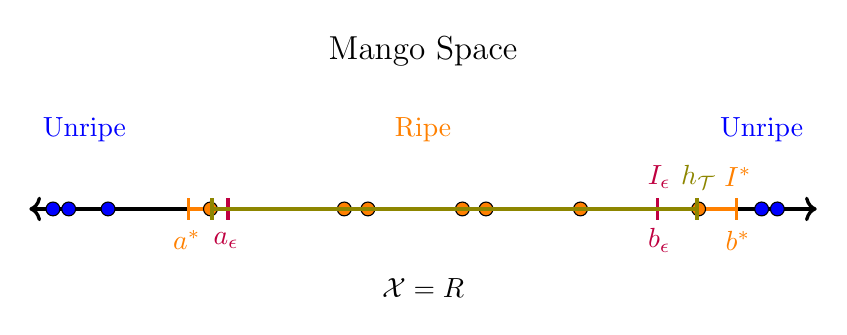
\begin{tikzpicture}
		\draw[<->,very thick] (-5,0) -- (5,0);
		\draw[color = orange, |-|,very thick] (-3,0) -- (4,0);
		\node[color=orange] at (4,.4) {$I^*$};
		\node at (0,2) {\large Mango Space} ;
		\node at (0,-1) {$\mathcal{X} = \mathbb{R}$} ;
		\node [color=blue] at (-4.3,1) {Unripe} ;
		\node [color=blue] at (4.3,1) {Unripe} ;
		\node [color=orange] at (0,1) {Ripe} ;

		\node [color=orange] at (-3,-.4) {$a^*$} ;
		\node [color=orange] at (4,-.4) {$b^*$} ;

		\draw [color=purple, |-|,very thick] (-2.5,0) -- (3,0);
		\node [color=purple] at (3,.4) {$I_\epsilon$} ;
		\node [color=purple] at (-2.5,-.4) {$a_\epsilon$} ;
		\node [color=purple] at (3,-.4) {$b_\epsilon$} ;



		\node[circle,draw=black, fill=orange, inner sep=0pt,minimum size=5pt] at (2,0) {};
		\node[circle,draw=black, fill=orange, inner sep=0pt,minimum size=5pt] at (-1,0) {};
		\node[circle,draw=black, fill=orange, inner sep=0pt,minimum size=5pt] at (-.7,0) {};
		\node[circle,draw=black, fill=orange, inner sep=0pt,minimum size=5pt] at (.5,0) {};
		\node[circle,draw=black, fill=orange, inner sep=0pt,minimum size=5pt] at (.8,0) {};
		\node[circle,draw=black, fill=orange, inner sep=0pt,minimum size=5pt] at (-2.7,0) {};
		\node[circle,draw=black, fill=orange, inner sep=0pt,minimum size=5pt] at (3.5,0) {};

		\node[circle,draw=black, fill=blue, inner sep=0pt,minimum size=5pt] at (-4.5,0) {};
		\node[circle,draw=black, fill=blue, inner sep=0pt,minimum size=5pt] at (-4,0) {};
		\node[circle,draw=black, fill=blue, inner sep=0pt,minimum size=5pt] at (-4.7,0) {};
		\node[circle,draw=black, fill=blue, inner sep=0pt,minimum size=5pt] at (4.3,0) {};
		\node[circle,draw=black, fill=blue, inner sep=0pt,minimum size=5pt] at (4.5,0) {};

		\draw [color=olive, |-|,very thick] (-2.7,0) -- (3.5,0);
   		\node [color=olive] at (3.5,.4) {$h_{\mathcal{T}}$} ;
	\end{tikzpicture}
  \end{minipage}
  \vfill
  \begin{minipage}[t][0.6\textheight][t]{\textwidth}
We have shown that if a randomly selected training set $\mathcal{T}$ of size $N$ contains a point in $[a^*,a_\epsilon]$ and a point in $ [b_\epsilon, b^*]$ than the ERM classifier must have total error less than $\epsilon$. What is the probability of this result \textbf{not} attaining?.\newline\pause

  \end{minipage}

\end{frame}






\begin{frame}[fragile]{}
  \begin{minipage}[t][0.4\textheight][t]{\textwidth}
	\centering
	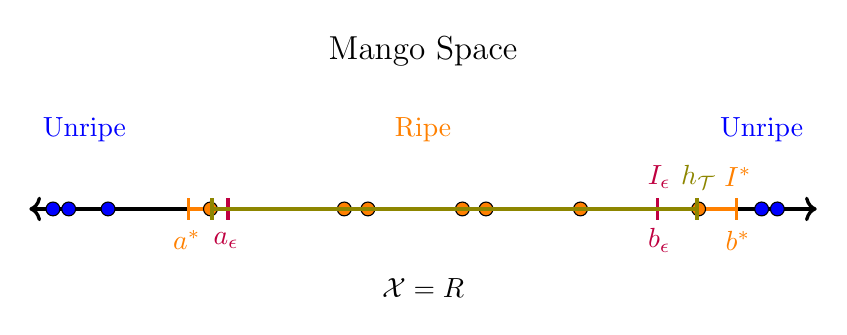
\begin{tikzpicture}
		\draw[<->,very thick] (-5,0) -- (5,0);
		\draw[color = orange, |-|,very thick] (-3,0) -- (4,0);
		\node[color=orange] at (4,.4) {$I^*$};
		\node at (0,2) {\large Mango Space} ;
		\node at (0,-1) {$\mathcal{X} = \mathbb{R}$} ;
		\node [color=blue] at (-4.3,1) {Unripe} ;
		\node [color=blue] at (4.3,1) {Unripe} ;
		\node [color=orange] at (0,1) {Ripe} ;

		\node [color=orange] at (-3,-.4) {$a^*$} ;
		\node [color=orange] at (4,-.4) {$b^*$} ;

		\draw [color=purple, |-|,very thick] (-2.5,0) -- (3,0);
		\node [color=purple] at (3,.4) {$I_\epsilon$} ;
		\node [color=purple] at (-2.5,-.4) {$a_\epsilon$} ;
		\node [color=purple] at (3,-.4) {$b_\epsilon$} ;



		\node[circle,draw=black, fill=orange, inner sep=0pt,minimum size=5pt] at (2,0) {};
		\node[circle,draw=black, fill=orange, inner sep=0pt,minimum size=5pt] at (-1,0) {};
		\node[circle,draw=black, fill=orange, inner sep=0pt,minimum size=5pt] at (-.7,0) {};
		\node[circle,draw=black, fill=orange, inner sep=0pt,minimum size=5pt] at (.5,0) {};
		\node[circle,draw=black, fill=orange, inner sep=0pt,minimum size=5pt] at (.8,0) {};
		\node[circle,draw=black, fill=orange, inner sep=0pt,minimum size=5pt] at (-2.7,0) {};
		\node[circle,draw=black, fill=orange, inner sep=0pt,minimum size=5pt] at (3.5,0) {};

		\node[circle,draw=black, fill=blue, inner sep=0pt,minimum size=5pt] at (-4.5,0) {};
		\node[circle,draw=black, fill=blue, inner sep=0pt,minimum size=5pt] at (-4,0) {};
		\node[circle,draw=black, fill=blue, inner sep=0pt,minimum size=5pt] at (-4.7,0) {};
		\node[circle,draw=black, fill=blue, inner sep=0pt,minimum size=5pt] at (4.3,0) {};
		\node[circle,draw=black, fill=blue, inner sep=0pt,minimum size=5pt] at (4.5,0) {};

		\draw [color=olive, |-|,very thick] (-2.7,0) -- (3.5,0);
   		\node [color=olive] at (3.5,.4) {$h_{\mathcal{T}}$} ;
	\end{tikzpicture}
  \end{minipage}
  \vfill
  \begin{minipage}[t][0.6\textheight][t]{\textwidth}
The probability of choosing $N$ training point i.i.d. from $\mathcal{D}$ and having either none in  $[a^*,a_\epsilon]$ or in $[b_\epsilon, b^*]$ is
$$
\mathcal{D}^N\bigg(\big\{\mathcal{T}\,:\,x_i\not\in [a^*,a_\epsilon],\,\forall \,i\big\}\cup\big\{\mathcal{T}\,:\,x_i\not\in [b_\epsilon, b^*],\,\forall \,i\big\}\bigg) \geq \delta\,.
$$
Every example of a training set that leads to a hypothesis class with true error great than $\epsilon$ can be found in the set above, so the probability of pulling $\mathcal{T}$ from that is at least $\delta$. We need to find an upper bound for this expression, and hence for the probability of pulling a non-representative training set. . 
  \end{minipage}

\end{frame}






\begin{frame}[fragile]{}
 \begin{minipage}[t][0.3\textheight][t]{\textwidth}
	\centering
	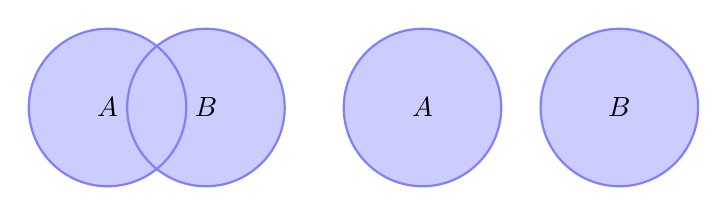
\begin{tikzpicture}
	\draw[fill=blue!20, draw=blue!50, thick] (0,0) circle (1cm) node {$A$} (0:1.25cm) circle (1cm) node {$B$};
	\draw[fill=blue!20, draw=blue!50, thick] (4,0) circle (1cm) node {$A$};
	\draw[fill=blue!20, draw=blue!50, thick] (6.5,0) circle (1cm) node {$B$};

\end{tikzpicture}
  \end{minipage}

Two facts from probability: 

\textbf{Union Bound}: The probability of the union is less than the sum of the probabilities
$$
\mathcal{D}(A\cup B) \leq \mathcal{D}(A) + \mathcal{D}(B)
$$

\textbf{Joint Probabilities}: For $x,y\sim \mathcal{D}$ independent, the probability $x\in A$ \textit{and} $y\in B$ is the product of the probabilities:
$$
\mathcal{D}(\{(x,y): x\in A\text{ and }y\in B\} ) = \mathcal{D}(\{x: x\in A\} ) \times \mathcal{D}(\{y: y\in B\} ) 
$$
\end{frame}






\begin{frame}[fragile]{}

By the union bound, 

  \begin{minipage}[t][0.6\textheight][t]{\textwidth}
\begin{align*}
\mathcal{D}^N&\bigg(\big\{\mathcal{T}\,:\,x_i\not\in [a^*,a_\epsilon],\,\forall \,i\big\}\cup\big\{\mathcal{T}\,:\,x_i\not\in [b_\epsilon, b^*],\,\forall \,i\big\}\bigg)
\\
&\leq
\mathcal{D}^N\bigg(\big\{\mathcal{T}\,:\,x_i\not\in [a^*,a_\epsilon],\,\forall \,i\big\}\bigg)+ \mathcal{D}^N\bigg(\big\{\mathcal{T}\,:\,x_i\not\in [b_\epsilon, b^*],\,\forall \,i\big\}\bigg)
\\
&=
\prod_{i=1}^N\mathcal{D}\bigg(\big\{x\,:\,x\not\in [a^*,a_\epsilon]\big\}\bigg) + \prod_{i=1}^N \mathcal{D}^N\bigg(\big\{x\,:\,x\not\in [b_\epsilon, b^*]\big\}\bigg)
\end{align*}
  \end{minipage}
Where we have used the i.i.d. assumption to notice that joint distribution is the same as the product of $N$ distributions. Now, lets bound each of these terms. 
\end{frame}





\begin{frame}[fragile]{}

Since 
$$
\mathcal{D}\bigg(\big\{x\,:\,x\not\in [a^*,a_\epsilon]\big\}\bigg) = 1 - \frac{\epsilon}2\,,
$$\pause
we can bound the probability by
\begin{align*}
\prod_{i=1}^N&\mathcal{D}\bigg(\big\{x\,:\,x\not\in [a^*,a_\epsilon]\big\}\bigg) + \prod_{i=1}^N \mathcal{D}^N\bigg(\big\{x\,:\,x_i\not\in [b_\epsilon, b^*]\big\}\bigg)
\\
&=
(1-\epsilon/2)^N + (1-\epsilon/2)^N 
\\
&\leq 2e^{-N\cdot\epsilon/2}
\end{align*}
\pause
The last is by Taylors approximation and is for connivance only. We have shown that 
$$
\delta\leq 2e^{-N\cdot\epsilon/2}\,.
$$
\end{frame}



\begin{frame}[fragile]{}
  \begin{minipage}[t][0.4\textheight][t]{\textwidth}
	\centering
	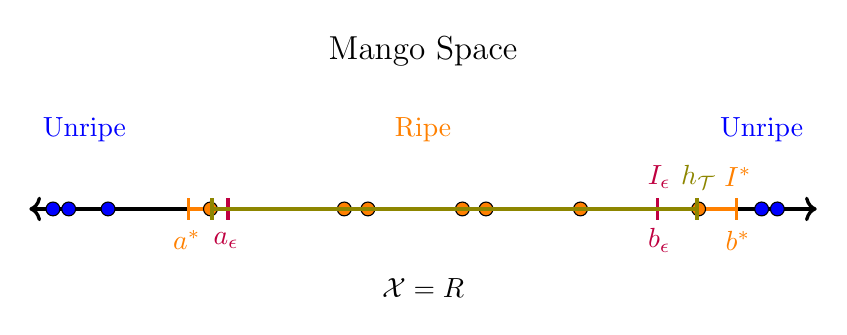
\begin{tikzpicture}
		\draw[<->,very thick] (-5,0) -- (5,0);
		\draw[color = orange, |-|,very thick] (-3,0) -- (4,0);
		\node[color=orange] at (4,.4) {$I^*$};
		\node at (0,2) {\large Mango Space} ;
		\node at (0,-1) {$\mathcal{X} = \mathbb{R}$} ;
		\node [color=blue] at (-4.3,1) {Unripe} ;
		\node [color=blue] at (4.3,1) {Unripe} ;
		\node [color=orange] at (0,1) {Ripe} ;

		\node [color=orange] at (-3,-.4) {$a^*$} ;
		\node [color=orange] at (4,-.4) {$b^*$} ;

		\draw [color=purple, |-|,very thick] (-2.5,0) -- (3,0);
		\node [color=purple] at (3,.4) {$I_\epsilon$} ;
		\node [color=purple] at (-2.5,-.4) {$a_\epsilon$} ;
		\node [color=purple] at (3,-.4) {$b_\epsilon$} ;



		\node[circle,draw=black, fill=orange, inner sep=0pt,minimum size=5pt] at (2,0) {};
		\node[circle,draw=black, fill=orange, inner sep=0pt,minimum size=5pt] at (-1,0) {};
		\node[circle,draw=black, fill=orange, inner sep=0pt,minimum size=5pt] at (-.7,0) {};
		\node[circle,draw=black, fill=orange, inner sep=0pt,minimum size=5pt] at (.5,0) {};
		\node[circle,draw=black, fill=orange, inner sep=0pt,minimum size=5pt] at (.8,0) {};
		\node[circle,draw=black, fill=orange, inner sep=0pt,minimum size=5pt] at (-2.7,0) {};
		\node[circle,draw=black, fill=orange, inner sep=0pt,minimum size=5pt] at (3.5,0) {};

		\node[circle,draw=black, fill=blue, inner sep=0pt,minimum size=5pt] at (-4.5,0) {};
		\node[circle,draw=black, fill=blue, inner sep=0pt,minimum size=5pt] at (-4,0) {};
		\node[circle,draw=black, fill=blue, inner sep=0pt,minimum size=5pt] at (-4.7,0) {};
		\node[circle,draw=black, fill=blue, inner sep=0pt,minimum size=5pt] at (4.3,0) {};
		\node[circle,draw=black, fill=blue, inner sep=0pt,minimum size=5pt] at (4.5,0) {};

		\draw [color=olive, |-|,very thick] (-2.7,0) -- (3.5,0);
   		\node [color=olive] at (3.5,.4) {$h_{\mathcal{T}}$} ;
	\end{tikzpicture}
  \end{minipage}
  \vfill
  \begin{minipage}[t][0.6\textheight][t]{\textwidth}
A bit of algebra shows the following: For any $\delta>0$ and any $\epsilon>0$, assume we have 
$$
N\geq \frac{2\log(2/\delta)}{\epsilon}
$$
points of the training data in $\mathcal{T}$. Then, with probability greater than $1-\delta$, the ERM rule returns a classifier $h_{\mathcal{T}}$ with total loss less than $\epsilon$.

We say then that with enough data, the output rule is \textbf{probably approximately correct}.
  \end{minipage}

\end{frame}







\begin{frame}[fragile]{}
The expression 
$$
N\geq \frac{2\log(2/\delta)}{\epsilon}
$$
provides a bound on the amount of data we need to have a high probability of getting a highly accurate result, \textit{given the assumptions} that the hypothesis class is $\mathcal{H} = \{\mathds{1}_I\,:\,I = [a,b]\}$ and that the data is actually generated by some $f\in H$. These are of course strong conditions and don't (yet) say anything about the accuracy of the classifier if the data is not drawn from $f$. \pause

But lets take a quick ``rule of thumb'' look at the result: 

\textbf{Question:} If I want to increase my accuracy by 50\%, how much must I increase by training set size? \pause

\textbf{Question:} If I want to increase my probability of getting a good training set by 50\%, how much must I increase the size by?
\end{frame}




\begin{frame}[fragile]{}
\textbf{Answer 1:}
$$
N\geq \frac{2\log(2/\delta)}{\frac{\epsilon}{2}} = 2\cdot \frac{2\log(2/\delta)}{\epsilon}\,.
$$
So decreasing error by a factor of $\alpha$ increases datasize by a factor of $\alpha$. \pause

\textbf{Answer 2:}
$$
N\geq \frac{2\log(2/\frac{\delta}{2})}{\epsilon} = \frac{2\log(2/\delta)}{\epsilon} + \frac{2\log(2)}{\epsilon}  \,.
$$
So increasing the probability of getting a good training sample is just a linear shift. 

This difference is very interesting: Practically it means that increasing the reliability of your classifier is easier than increasing its accuracy. 

\end{frame}









\section{PAC and APAC Learning}

\begin{frame}[fragile]{PAC Learnability}
  \begin{minipage}[t][0.4\textheight][t]{\textwidth}
	\centering
	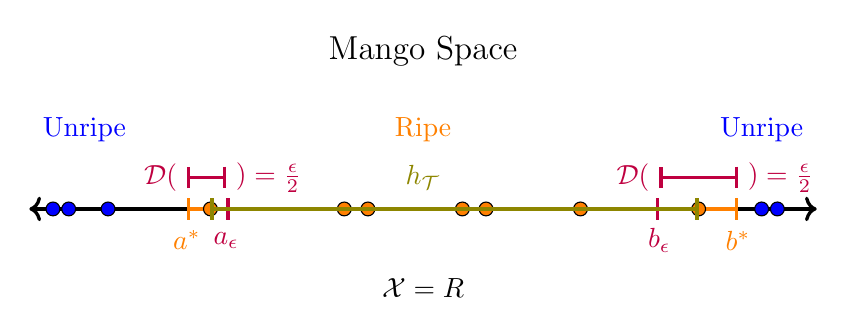
\begin{tikzpicture}
		\draw[<->,very thick] (-5,0) -- (5,0);
		\draw[color = orange, |-|,very thick] (-3,0) -- (4,0);
		\node at (0,2) {\large Mango Space} ;
		\node at (0,-1) {$\mathcal{X} = \mathbb{R}$} ;
		\node [color=blue] at (-4.3,1) {Unripe} ;
		\node [color=blue] at (4.3,1) {Unripe} ;
		\node [color=orange] at (0,1) {Ripe} ;

		\node [color=orange] at (-3,-.4) {$a^*$} ;
		\node [color=orange] at (4,-.4) {$b^*$} ;

		\visible<5->{
		\draw [color=purple, |-|,very thick] (-2.5,0) -- (3,0);
		\node [color=purple] at (-2.5,-.4) {$a_\epsilon$} ;
		\node [color=purple] at (3,-.4) {$b_\epsilon$} ;
		
		\draw [color=purple, |-|,very thick] (-3,.4)-- (-2.5,.4);
		\draw [color=purple, |-|,very thick] (3,.4)--(4,.4);
		\node [left, color=purple] at (-3,.4) {$\mathcal{D}( $} ;
		\node [right, color=purple] at (-2.5,.4) {$)  = \frac{\epsilon}{2}$} ;
		\node [left, color=purple] at (3,.4) {$\mathcal{D}( $} ;
		\node [right, color=purple] at (4,.4) {$)  = \frac{\epsilon}{2}$} ;
		

		}


		\visible<2->{
		\node[circle,draw=black, fill=orange, inner sep=0pt,minimum size=5pt] at (2,0) {};
		\node[circle,draw=black, fill=orange, inner sep=0pt,minimum size=5pt] at (-1,0) {};
		\node[circle,draw=black, fill=orange, inner sep=0pt,minimum size=5pt] at (-.7,0) {};
		\node[circle,draw=black, fill=orange, inner sep=0pt,minimum size=5pt] at (.5,0) {};
		\node[circle,draw=black, fill=orange, inner sep=0pt,minimum size=5pt] at (.8,0) {};
		\node[circle,draw=black, fill=orange, inner sep=0pt,minimum size=5pt] at (-2.7,0) {};
		\node[circle,draw=black, fill=orange, inner sep=0pt,minimum size=5pt] at (3.5,0) {};

		\node[circle,draw=black, fill=blue, inner sep=0pt,minimum size=5pt] at (-4.5,0) {};
		\node[circle,draw=black, fill=blue, inner sep=0pt,minimum size=5pt] at (-4,0) {};
		\node[circle,draw=black, fill=blue, inner sep=0pt,minimum size=5pt] at (-4.7,0) {};
		\node[circle,draw=black, fill=blue, inner sep=0pt,minimum size=5pt] at (4.3,0) {};
		\node[circle,draw=black, fill=blue, inner sep=0pt,minimum size=5pt] at (4.5,0) {};}

		\visible<3->{
		\draw [color=olive, |-|,very thick] (-2.7,0) -- (3.5,0);
   		\node [color=olive] at (0,.4) {$h_{\mathcal{T}}$} ;}
	\end{tikzpicture}
  \end{minipage}
  \vfill
  \begin{minipage}[t][0.6\textheight][t]{\textwidth}
We have shown that for a sufficiently large training set $\mathcal{T}$, the \textbf{ERM} rule on the hypothesis class of interval classifiers, $\mathcal{H}$, outputs a classifier $h_{\mathcal{T}}$ that is \textbf{probably approximately correct} or \textbf{PAC}. \newline

\visible<4->{That is, if the inputs have distribution $\mathcal{D}$ and $f$ is the true labeling, then the error $L_{(\mathcal{D},f)}(h_{\mathcal{T}})<\epsilon$ with probability $1-\delta$, provided
$$
N > 2\frac{\log(2/\delta)}{\epsilon}\,.
$$}
  \end{minipage}


\end{frame}





\begin{frame}[fragile]{PAC Learnability}


\textbf{PAC Learnability:} A hyptothesis class $\cH$ is PAC learnable if there exists a function $N_{\mathcal{H}}:(0,1)^2\to \mathbb{N}$ and a learning algorithm $A$ with the following properties:\newline

For every $\epsilon, \delta\in (0,1)$, and for every distribution $\mathcal{D}$ on $\cX$, and for every labeling function $f:\cX\to \cY$, if realizability holds, then with probability at least $1-\delta$, $A(\cT) = h$ has total error $L_{(\cD,f)}(h)<\epsilon$ provided $|\cT|>N_{\cH}(\epsilon, \delta)$.
\end{frame}




\begin{frame}[fragile]{PAC Learnability}


\textbf{PAC learnability} has two parameters: 

\begin{itemize}
\item[] The \textbf{accuracy parameter} $\epsilon$ bounds the total error of the output classifier.\pause
\item[] The \textbf{confidence parameter} $\delta$ indicates how likely the classifier is to make the accuracy requirement. \pause
\end{itemize}

The stochastic nature of the definition reflects the fact that there is always some chance of choosing a highly non-representative data sample from $\mathcal{D}$. 

\end{frame}





\begin{frame}[fragile]{Sample Complexity}


The function $N_{\cH}:(0,1)^2\to \bR$ is called the \textbf{sample complexity} of learning $\cH$. It governs the number of examples needed to learn $\cH$. \newline

Note, that if $\cH$ is PAC learnable there are actually many functions $N_\cH$ that satisfy the requirements of PAC learnability. In general, we will use sample complexity to refer to the minimum such function in the class of all $N_\cH$. 



\end{frame}



\begin{frame}[fragile]{Sample Complexity for Interval Indicators}

We can restate our result about the interval classifier in the PAC framework in terms of the sample complexity:

Our computation in before showed that the hypothesis class of integer indicator functions 
$$
\mathcal{H} = \{\mathds{1}_{I}\,:\,I = [a,b],\, a,b\in \bR\}
$$ 
is PAC learnable, with sample complexity
$$
N_\cH(\epsilon,\delta) \leq \text{ceil}\left(\,2\frac{\log(2/\delta)}{\epsilon}\,\right)\,.
$$



\end{frame}













%%%%%%%%%%%%%% Agnostic PAC Learning %%%%%%%%%%%%%% 

\begin{frame}[fragile]{Realizability Revisited}

In many practical problems, the assumption of realizability does not hold. Recall that formally, realizability is the assumption that there exists an $h^*\in \cH$ such that 
$$
\bP_{X\sim \cD}(\,h^*(X) = f(X)\,) = 1\,.
$$
Realizability can fail in two ways:
\begin{itemize}
\item[] The labels could be generated by a function $f$ ``far away" from $\cH$. 
\item[] The labels may not be fully determined by the features. 
\end{itemize}

We will now drop the notion of a labeling function $f$ and instead assume the data labels are generated by a distribution. 

\end{frame}




\begin{frame}[fragile]{Joint Distribution}
  \begin{minipage}[t][0.5\textheight][t]{\textwidth}
    \includegraphics[height=0.5\textheight]{L3JointDist1.png}
        \centering
  \end{minipage}
  \vfill
  \begin{minipage}[t][0.5\textheight][t]{\textwidth}
Let $\cD$ be a joint distribution over the space of points and labels $\cX\times\cY$. $\cD$ can thought of as being composed of two parts: \pause
\begin{itemize}
\item[] The \textbf{marginal} distribution $\cD_X$, which gives the likelihood of a point of $\cX$ being sampled.\pause
\item[] The \textbf{conditional} distribution $\cD(Y|X = x)$, which give the likelyhood of a label given that $x$ was sampled. 
\end{itemize}
  \end{minipage}
\end{frame}


\begin{frame}[fragile]{Joint Distribution}
  \begin{minipage}[t][0.5\textheight][t]{\textwidth}
    \includegraphics[height=0.5\textheight]{L3JointDist2.png}
        \centering
  \end{minipage}
  \vfill
  \begin{minipage}[t][0.5\textheight][t]{\textwidth}
Let $\cD$ be a joint distribution over the space of points and labels $\cX\times\cY$. As we saw before, $\cD$ can thought of as being composed of two parts: 
\begin{itemize}
\item[] The \textbf{marginal} distribution $\cD_X$, which gives the likelihood of a point of $\cX$ being sampled.
\item[] The \textbf{conditional} distribution $\cD(Y|X = x)$, which give the likelyhood of a label given that $x$ was sampled. 
\end{itemize}
  \end{minipage}
\end{frame}




\begin{frame}[fragile]{Joint Distribution}
  \begin{minipage}[t][0.5\textheight][t]{\textwidth}
    \includegraphics[height=0.5\textheight]{L3JointDist3.png}
        \centering
  \end{minipage}
  \vfill
  \begin{minipage}[t][0.5\textheight][t]{\textwidth}
Let $\cD$ be a joint distribution over the space of points and labels $\cX\times\cY$. As we saw before, $\cD$ can thought of as being composed of two parts: 
\begin{itemize}
\item[] The \textbf{marginal} distribution $\cD_X$, which gives the likelihood of a point of $\cX$ being sampled.
\item[] The \textbf{conditional} distribution $\cD(Y|X = x)$, which give the likelyhood of a label given that $x$ was sampled. 
\end{itemize}
  \end{minipage}
\end{frame}





\begin{frame}[fragile]{Error}
Given a joint distribution on $\cX\times \cY$, the \textbf{true error} (\textbf{risk}) of a predictor $h$ under the 1-Accuracy loss is 
\begin{flalign*}
\hspace{2em} L_{\cD}(h):= \bP_{(X,Y)\sim \cD}\,\big[h(X)\neq Y \big] \,,&&
\end{flalign*}
or
\begin{flalign*}
\hspace{2em} L_{\cD}(h):= \cD\Big(\,\big\{(X,Y)\,:\,h(X)\neq Y\big\}\,\Big)\,.&&
\end{flalign*}\pause
The \textbf{empirical risk} remains the same,
\begin{flalign*}
\hspace{2em} L_{\cT}(h):= \frac{|\{i\,:\, h(x_i)\neq y_i\}|}{N}\,.&&
\end{flalign*}\pause
The goal now will be to find some classifier $h:\mathcal{X}\to\mathcal{Y}$ that (probably approximately) minimizes the \textbf{true risk} $L_{\cD}(h)$. 
\end{frame}








\begin{frame}[fragile]{Bayes Optimal Predictor}
Given any probability distribution $\cD$ over $\cX\times\{0,1\}$, the ``best'' (measured by $L_{\cD}(h)$ minimizing) possible label predicting function from $\cX$ to $\{0,1\}$ will be
$$
f_{\cD} = \begin{cases}
1 & \text{if }\bP[Y=1|X=x]\geq 1/2\,,
\\
0 &\text{otherwise}.
\end{cases}
$$
This function is known as the \textbf{Bayes optimal predictor}. It's a good exercise to show that for any other classifier $g$, $L_{\cD}(f^*)\leq L_{\cD}(g)$. 
\end{frame}





\begin{frame}[fragile]{Bayes Optimal Predictor}
  \begin{minipage}[t][0.5\textheight][t]{\textwidth}
    \begin{overprint}
    \onslide<1|handout:0>   \centering \includegraphics[height=0.5\textheight]{L3JointDist3.png}
    \onslide<2,3|handout:1>   \centering\includegraphics[height=0.5\textheight]{L3JointDist4.png}
    \end{overprint}
  \end{minipage}
  \vfill
  \begin{minipage}[t][0.5\textheight][t]{\textwidth}
For example, given the conditional probability for our simulated mango distribution, the Bayes optimal predictor simply selects the most likely labeling for each data point.\pause\pause\newline

Of course, the Bayes optimal predictor ``knows" the underlying distrbiution, while the PAC learner does not. 
  \end{minipage}
\end{frame}




\begin{frame}[fragile]{Agnostic PAC Learnability}
\textbf{Agnostic PAC Learnability:} A hypothesis class $\cH$ is agnostic PAC learnable if there exists a function $N_{\mathcal{H}}:(0,1)^2\to \mathbb{N}$ and a learning algorithm $A$ with the following properties:\newline\pause

For every $\epsilon, \delta\in (0,1)$, and for every distribution $\mathcal{D}$ on $\cX\times\cY$, when running $A$ on a training set of $N\geq N_\cH(\delta,\epsilon)$ i.i.d. samples, then, with probability at least $1-\delta$, the total error of $A(\cT) = h$ is bounded by
$$
L_{\cD}(h)\leq\min_{h'\in \mathcal{H}}\,L_{\cD}(h')+\epsilon\,.
$$ 
\pause\newline

(Of course, if realizability holds $\min_{h'\in \mathcal{H}}\,L_{\cD}(h') = 0$.)
\end{frame}



\begin{frame}[fragile]{Agnostic PAC Learnability}
\textbf{Agnostic PAC Learnability:} If the realizability assumption does not hold, no learner can guarantee an arbitrarily small error. Instead, we declare the learner a success if the error is not must larger than the best achievable error within the hypothesis class $\mathcal{H}$.\pause

APAC learnability can be extended to more generalized losses on more generalized sets. For example,  clustering algorithms replace $\mathcal{X}$ and $\mathcal{Y}$ with a single space $\mathcal{Z}$, with a loss set by an internal metric. In fact, we usually write $\mathcal{Z} = \mathcal{X}\times \mathcal{Y}$ to include more general notions of loss on even labeled data. 
\end{frame}






\begin{frame}[fragile]{Agnostic PAC Learnability with Generalized Loss}
\textbf{Agnostic PAC With Loss:} A hypothesis class $\cH$ is agnostic PAC learnable with resepct to a set $\cZ$ and loss $\ell:\cH\times \cZ\to \bR_+$ if there exists a function $N_{\mathcal{H}}:(0,1)^2\to \mathbb{N}$ and a learning algorithm $A$ with the following properties:\newline\pause

For every $\epsilon, \delta\in (0,1)$, and for every distribution $\mathcal{D}$ on $\cZ$, when running $A$ on a training set of $N\geq N_\cH(\delta,\epsilon)$ i.i.d. samples, then, with probability at least $1-\delta$, the total error of $A(\cT) = h$ is bounded by
$$
L_{\cD}(h)\leq\min_{h'\in \mathcal{H}}\,L_{\cD}(h')+\epsilon\,,
$$ 
where $L_{\cD}(h) = E_{z\sim\cD}\big[\ell(h,Z)\big]$.\pause

We will this criteria \textbf{APAC learnable}. 
\end{frame}







%%%%%%%%%%%%%% Uniform Convergence %%%%%%%%%%%%%% 

\section{Proving Bounds in APAC}

\begin{frame}[fragile]{Proving Bounds in APAC}
\textbf{Goal:} Prove that every finite hypothesis class is APAC learnable. \newline\pause

To work in the APAC framework we need some tools: 

\begin{itemize}
\item[] \textbf{Uniform convergence} - gives criteria for APAC learnability.
\item[] \textbf{Hoeffding's Inequality} - computes sample complexity from the generalized loss. 
\end{itemize}


\end{frame}


\section{Uniform Convergence}

\begin{frame}[fragile]{$\mathbf{\epsilon}$-Representative Training Sets}
If a hypothesis class is APAC learnable, running $ERM(h)$ on a training set $\mathcal{T}$ will minimize the true error.\newline

It suffices to ensure that the empirical risk $L_\cT(h)$ is a good indicator of the true risk $L_\cD(h)$ for all $h\in \cH$. \pause

A training set $\mathcal{T}$ is called \textbf{$\mathbf{\epsilon}$-representative} (w.r.t. $\cZ$, $\cH$, $\ell$ and $\cD$) if
$$
\forall h\in \mathcal{H},\,\,\, |L_\cT(h) - L_\cD(h)|\leq \epsilon\,,
$$\pause
that is, if empirical risk on $\cT$ is a good indicator of the true risk on $\cZ$. 

\end{frame}




\begin{frame}[fragile]{$\mathbf{\epsilon}$-Representative Training Sets}
\textbf{Lemma:} If a training set is $\epsilon/2$-representative, then any output of $ERM_\cH(\cT)$ (that is any $h_\cT\in \text{argmin}_{h\in\cH}L_\cT(h)$) satisfies 
$$
L_\cD(h_\cT) \leq \min_{h\in \cH}\, L_\cD(h) + \epsilon\,.
$$\pause

\textbf{Proof:} For every $h\in \cH$, 
$$
L_\cD(h_\cT)  \underset{\epsilon-rep}{\leq} L_\cT(h_\cT) + \frac\epsilon2 \pause \underset{ERM}{\leq}  L_\cT(h) + \frac\epsilon2  \pause \underset{\epsilon-rep}{\leq}  L_\cD(h) + \epsilon\,.
$$
\hspace*{\fill}$\Box$

\end{frame}



\begin{frame}[fragile]{Uniform Convergence}
\textbf{Uniform Convergence:} A hypothesis class has the uniform convergence property (w.r.t. $Z$ and $\ell$) if there exists a function $N^{UC}_\cH:(0,1)^2\to\mathbb{N}$ such that for every $\epsilon,\delta \in (0,1)$, if $\cT$ is a training set of size $N\geq N^{UC}_\cH(\epsilon, \delta)$ then, with a probability of at least $1-\delta$ it is $\epsilon$-representative.\newline\pause

\textbf{Corollary:} If a class has the uniform convergence property, then it is APAC learnable by ERM with sample complexity $N^{UC}_\cH$.

\end{frame}



%%%%%%%%%%%%%% Hoeffding's Inequality %%%%%%%%%%%%%% 
\section{Hoeffding's Inequality}

\begin{frame}[fragile]{Hoeffding's Inequality}
We now have a criteria for APAC learnability in terms of the sample sets $\cT$, but we need some tools from probability to estimate expectation values. \newline\pause

\textbf{Hoeffding's Inequality:} Let $\theta_1,\ldots, \theta_N$ be i.i.d. random variables with $\bP[a\leq \theta\leq b] = 1$. Define $\theta = \sum \theta_i$. Then for any $\epsilon>0$, 
$$
\bP\left[\, \left|\frac{1}{N} \sum_{i=1}^N(\theta_i - E[\theta_i]\,)\right|>\epsilon  \,\right]\leq 2\exp\left(-2N\epsilon^2/(b-a)^2\right)\,.
$$
\end{frame}



\begin{frame}[fragile]{Hoeffding's Inequality}
\textbf{Hoeffding's Inequality:} Let $\theta_1,\ldots, \theta_N$ be i.i.d. random variables with $\bP[a\leq \theta\leq b] = 1$. Define $\theta = \sum \theta_i$. Then for any $\epsilon>0$, 
$$
\visible<4->{\delta} = \bP\left[\, \left|\frac{1}{N} \sum_{i=1}^N(\theta_i - E[\theta_i]\,)\right|>\epsilon  \,\right]\leq 2\exp\left(-2N\epsilon^2/(b-a)^2\right)\,.
$$
\rule{\textwidth}{0.4pt}\pause

\textbf{Relation to APAC:} Setting $\theta_i = \ell(h,z_i)$ immediately gives 
$$
L_\cT(h) = \frac{1}{N} \sum_{i=1}^N \ell(h,z_i) =  \frac{1}{N} \sum_{i=1}^N \theta_i\,,\pause
$$ 
and $L_\cD(h) = \frac{1}{N} \sum_{i=1}^N E[\theta_i] = E[\ell(h,z)]$. \pause So 
$$
\delta = \cD\Big(\,\big\{\mathcal{T}:|L_\cT(h) - L_\cD(h)|>\epsilon\big\}\Big)\,.
$$

\end{frame}





%%%%%%%%%%%%%% Finite Model Spaces are PAC Learnable %%%%%%%%%%%%%% 
\section{Finite Hypothesis Classes are APAC Learnable}


\begin{frame}[fragile]{Finite Hypothesis Classes are APAC Learnable}
We are in a position to prove our first big theorem. The fact that finite hypothesis classes are APAC learnable is an important yardstick in machine learning both as a theoretical comparison and because practically our hypothesis classes aren't infinite.\newline\pause

For example, $\mathcal{H}$ could be the set of predictors that can be implement in $10^{10}$ bits in Python. Our mango example is infinite, but if we discretize it (say by encoding the color and softness parameters as 64 bit floats) it becomes finite. \pause\newline

In fact, any time we discretize the data, the set of all functions $h:\mathcal{X}\to\mathcal{Y}$ be comes finite. However, this doesn't necessarily fix things for us; as we just saw accuracy isn't cheap.
\end{frame}



\begin{frame}[fragile]{Finite Hypothesis Classes are APAC Learnable}
\textbf{Finite Hypothesis Classes are APAC Learnable:}
Let $(\mathcal{Z},\cD,\ell)$ be a domain, distribution and loss function and let $\cH$ be a finite hypothesis class. Fix $\epsilon,\delta\in (0,1)$. \pause 

By uniform convergence, we need to find a sample size $N$ the guarantees (with probability at least $1-\delta$) that if $|\mathcal{T}|>N$, for all $h\in \mathcal{H}$, 
$$
|L_\cT(h) - L_\cD|\leq \epsilon.
$$
\pause 
This is equivalent to showing
$$
\cD^N\Big(\big\{\cT:\exists h\in \mathcal{H}\,,|L_\cT(h)-L_\cD(h)|>\epsilon\big\}\Big)<\delta\,.
$$ 
\end{frame}



\begin{frame}[fragile]{Finite Hypothesis Classes are APAC Learnable}
\textbf{Finite Hypothesis Classes are APAC Learnable:}
Let $(\mathcal{Z},\cD,\ell)$ be a domain, distribution and loss function and let $\cH$ be a finite hypothesis class. Fix $\epsilon,\delta\in (0,1)$. 

By uniform convergence, we need to find a sample size $N$ the guarantees (with probability at least $1-\delta$) that $h\in \mathcal{H}$, 
$$
|L_\cT(h) - L_\cD|\leq \epsilon.
$$
This is equivalent to showing
$$
\cD^N\Big(\,\boxed{\big\{\cT:\exists h\in \mathcal{H}\,,|L_\cT(h)-L_\cD(h)|>\epsilon\big\}}\,\Big)<\delta\,.
$$ 
Lets describe the set of bad training sets. 
\end{frame}




\begin{frame}[fragile]{Finite Hypothesis Classes are APAC Learnable}
The set of bad training sets can be written as the union of the bad sets for each $h$: 
$$
\big\{\cT:\exists h\in \mathcal{H}\,,|L_\cT(h)-L_\cD(h)|>\epsilon\big\} = \bigcup_{h\in\cH} \big\{\cT:|L_\cT(h)-L_\cD(h)|>\epsilon\big\}\,.
$$\pause
We then use the union bound to write
\begin{align*}
\cD^N\Big(\big\{\cT:\exists h\in \mathcal{H}\,,&|L_\cT(h)-L_\cD(h)|>\epsilon\big\}\Big)
\\
&\leq \sum_{h\in\cH}\cD^N\Big(\big\{\cT:\mathcal{H}\,,|L_\cT(h)-L_\cD(h)|>\epsilon\big\}\Big)\,.
\end{align*}
\end{frame}




\begin{frame}[fragile]{Finite Hypothesis Classes are APAC Learnable}
Let $\theta_i = \ell(h,z_i)$. Since $h$ is fixed and $z_i$ are i.i.d., $\theta_i$ are also i.i.d.. As before, $L_\cT(h) = \frac{1}{N}\sum\theta_i$ and $L_\cD(h) = E[\ell(h,z_i)] = \mu$. Finally, for simplicity, lets assume that the range of $\ell$ is $[0,1]$. \pause Hoeffding's inequality gives that for any $h\in \cH$,
\begin{align*}
\cD^N\Big(\big\{\cT:\mathcal{H}\,,|L_\cT(h)-L_\cD(h)|>\epsilon\big\}\Big) 
= \bP\left[\left| \frac{1}{N}\sum_{i=1}^N\theta_i-\mu \right|>\epsilon\right] \leq 2e^{-2N\epsilon^2}\,.
\end{align*}\pause
Summing over the contributions for all $h\in \cH$ yields
\begin{align*}
\cD^N\Big(\big\{\cT:\exists h\in \mathcal{H}\,,|L_\cT(h)-L_\cD(h)|>\epsilon\big\}\Big)&\leq \sum_{h\in\cH}2e^{-2N\epsilon^2}
\\
&=2|\cH|e^{-2N\epsilon^2}\,.
\end{align*}
\end{frame}




\begin{frame}[fragile]{Finite Hypothesis Classes are APAC Learnable}
Therefore, if we choose
\begin{align*}
N\geq \frac{\log(2|\cH|/\delta)}{2\epsilon^2}\,,
\end{align*}
then 
\begin{align*}
\cD^N\Big(\big\{\cT:\exists h\in \mathcal{H}\,,|L_\cT(h)-L_\cD(h)|>\epsilon\big\}\Big)<\delta\,.\,\,\,\Box
\end{align*}
\end{frame}



\begin{frame}[fragile]{Finite Hypothesis Classes are APAC Learnable}
\textbf{Finite Hypothesis Classes are APAC Learnable:}
We have shown that $\mathcal{H}$ enjoys the uniform convergence property with
$$
N_{\cH}^{UC}(\epsilon,\delta)\leq \text{ceil }\left(\frac{\log(2|\cH|/\delta)}{2\epsilon^2}\right)\,.
$$\pause
Therefore, the class is APAC learnable using ERM with sample complexity 
$$
N_{\cH}(\epsilon,\delta)\leq N_{\cH}^{UC}(\epsilon/2,\delta) \leq \text{ceil }\left(\frac{2\log(2|\cH|/\delta)}{\epsilon^2}\right)\,.
$$
\end{frame}



\begin{frame}[fragile]{Discretizing}
As a final note, we can discretize a infinite hypothesis class to get a rough bound on the complexity. \pause For example, each function in the class of interval indicators $I_{[a,b]}$ depends on two real parameters $a,b\in \bR$ which we could represent as, say, 64 bit floats. In general, if we represent $d$ parameters as $b$ bit floats, there are at most
$$
2^{d\times b}
$$
such functions in $\cH$. \pause Applying the bound for finite classes, the sample complexity is at most
$$
N\leq \frac{b\cdot d \log 4+2\log(2/\delta)}{\epsilon^2}\,.
$$
The sample complexity is linear in the number of parameters. 

\end{frame}




\section{Deriving Hoeffding's Inequality}


\begin{frame}[fragile]{Markov’s Inequality}
Hoeffdings inequality is a powerful, but complicated bound. We will start with \textbf{Markov} and \textbf{Chebyshev}'s inequalities as estimates for probabilties of the form
$$
\bP\big[ f(\theta)>\epsilon \big]\,.
$$\pause
We will then define the exponential \textbf{moment generating function} to extend these results to sums of random variables
$$
\bP\big[ \sum_i f(\theta_i)>\epsilon \big]\,.
$$\pause
We finally define \text{Hoeffding's Lemma} to bound exponential probabilities.

\end{frame}



\begin{frame}[fragile]{Markov’s Inequality}
\textbf{Markov’s inequality:} Let $\theta\geq 0$ be a random variable on $\mathbb{R}_+$. Then, for all $\epsilon\geq 0$, 
$$
\bP(\theta\geq \epsilon)\leq \frac{E[\theta]}\epsilon\,.
$$\pause
\textbf{Proof:}
\[
  \begin{aligned}
  \action<+->{E[\theta] &= \int_{\bR_+}\theta p(\theta)d\theta & \\}
  \action<+->{&\geq \int_{\epsilon}^\infty\theta p(\theta)d\theta &\hspace{5em} &\text{since $p(\theta)\geq0$}\\}
  \action<+->{&\geq \int_{\epsilon}^\infty \epsilon p(\theta)d\theta & &\text{since $\theta>\epsilon$}\\}
  \action<+->{&= \epsilon\bP(\theta>\epsilon)\,. &&\Box}
  \end{aligned}
\]
\action<+->{Many probability estimates are just extensions are Markov's inequality.}

\end{frame}



\begin{frame}[fragile]{Chebyshev’s Inequality}
\textbf{Chebyshev’s inequality:} Let $\theta\geq 0$ be a random variable on $\mathbb{R}$ with $\text{Var}(\theta)<\infty$. Then
\[
\bP(\,|\theta - E[\theta] |\,\geq \epsilon)\leq \frac{\text{Var}[\theta]}{\epsilon^2}\,.
\]\pause
\textbf{Proof:} This is a direct appliction of Markov's inequality:
\[
  \begin{aligned}
  \action<+->{ \bP(\,|\theta - E[\theta]|\,\geq \epsilon) &= \bP\Big((\theta - E[\theta])^2\geq \epsilon^2\Big) \\}
  \action<+->{&\leq \frac{E\big[\,(\theta - E[\theta])^2\big]}{\epsilon^2} \,.\,\,\Box }
  \end{aligned}
\]\action<+->{As a side note, one nice consequence of Chebyshev’s inequality is that the averages of random variables converge to their mean. This is one face of the \textbf{law of large numbers}.}

\action<+->{\textbf{Exercise:} For $\theta_i$ i.i.d, with $E(\theta_i)=0$, show that $\text{Var}(\theta) = \frac1N\text{Var}(\theta_i)$.}

\end{frame}





\begin{frame}[fragile]{Moment generating functions}
For a real random variable $\theta$, the \textbf{moment generating function} is the exponential 
$$
M_\theta(\lambda) := E[e^{\lambda \theta}]\,.
$$ \pause
Taking the expectation the exponential we can read the moments off of $M_\theta(\lambda)$:
$$
M_\theta(\lambda) = 1 +\lambda E(X) + \frac{\lambda^2}{2}E(X^2) + \ldots
$$

\end{frame}




\begin{frame}[fragile]{Moment generating functions}
Moment generating functions play particularly nicely with sums of random variables, turning them into products: for $\theta_i$ i.i.d.,
\[
M_{\theta_1+\ldots+\theta_N}(\lambda) = E\left( e^{\lambda(\theta_1+\ldots+\theta_N)} \right) = \prod_{i=1}^N M_{\theta_i}(\lambda)\,.
\]
\pause Crucially, by mononicity,
$$
\bP(\theta\geq \epsilon) = \bP\left(e^\theta \geq e^\epsilon\right)\,,
$$
so we can recast probability inequalities in terms of exponential functions!

\end{frame}












\begin{frame}[fragile]{Hoeffding's Lemma}
Finally, we want to bound $E(e^{\lambda \theta})$.\newline

\textbf{Hoeffding's Lemma:} Let $X$ be a random variable on $[a,b]$ with $E(X)=0$. Then for all $\lambda>0$, 
$$
E(e^{\lambda X}) \leq e^{\frac{\lambda^2(b-a)^2 }8}
$$\pause
\textbf{Proof:} Since $e^x$ is convex on $[a,b]$, $$e^{\lambda X} \leq te^{\lambda a} + (1-t)e^{\lambda b} $$
for all $t\in(0,1)$. \pause Setting $t = \frac{b-x}{b-a}$ and taking expectation value we find
$$
E(e^{\lambda X})  \leq \frac{b-E(X)}{b-a}e^{\lambda a} + \frac{E(X)-a}{b-a}e^{\lambda b} = \frac{b}{b-a}e^{\lambda a} - \frac{a}{b-a}e^{\lambda b}\,.
$$
This last function can be bounded by Taylor approximation, giving the result. $\Box$

\end{frame}







\begin{frame}[fragile]{Hoeffding's Inequality}
Now that we have the tools, lets recall the statement of Hoeffding's inequality:

\textbf{Hoeffding's Inequality:} Let $\theta_1,\ldots, \theta_N$ be i.i.d. random variables with $\bP[a\leq \theta\leq b] = 1$. Define $\theta = \sum \theta_i$. Then for any $\epsilon>0$, 
$$
\delta = \bP\left[\, \left|\frac{1}{N} \sum_{i=1}^N(\theta_i - E[\theta_i]\,)\right|>\epsilon  \,\right]\leq 2\exp\left(-2N\epsilon^2/(b-a)^2\right)\,.
$$
\end{frame}




\begin{frame}[fragile]{Proof of Hoeffding's Inequality}
\textbf{Proof:} Let $X_i = \theta_i - E[\theta_i]$ and $X = \frac1N\sum_{i=1}^N X_i$. \pause By Markov's inequality,
$$
\bP[X\geq \epsilon] = \bP\left[ e^{\lambda X} \geq e^{\lambda \epsilon} \right] \leq E[e^{\lambda X}]e^{-\lambda \epsilon }
$$\pause
Since the $X_i$'s are i.i.d., 
$$
E[e^{\lambda X}] = \prod_{i=1}^N E\left[e^{\frac{\lambda X_i}N}\right]\pause
\leq
\prod_{i=1}^N e^{\frac{\lambda^2(b-a)^2 }{8N^2}} = e^{\frac{\lambda^2(b-a)^2 }{8N}}
$$
by Hoeffding's Lemma. \pause Combining these results and setting $\lambda = 4N\epsilon/(b-a)^2$ gives
$$
\bP[X\geq \epsilon] \leq  \exp\left(-2N\epsilon^2/(b-a)^2\right)\,.
$$
Repeating the above for $\bP[X\leq -\epsilon] $ and adding the results completes the proof. $\Box$
\end{frame}








\begin{frame}[fragile]{Hoeffding's Inequality}
A little bit of algebra allows us to write the following:\newline

\textbf{Hoeffding's Inequality II:} If we choose 
$$
N \geq \frac{(b-a)^2}{2\epsilon^2}\log \frac{2}{\delta}\,,
$$
then, with probability $1-\delta$, the difference between the empirical mean $\frac{1}{N}\sum_{i=1}^N \theta_i$ and the true mean $E(\theta)$ is less than $\epsilon$. \pause

In a very general sense this is telling us about the relative ``cost" of accuracy $\epsilon$ vs confidence $\delta$. In short, accuracy is expensive, while confidence is cheap.
\end{frame}





\begin{frame}[fragile]{Hoeffding's Inequality}
For example, according to
$$
N \geq \frac{(b-a)^2}{2\epsilon^2}\log \frac{2}{\delta}\,,
$$
if we want to increase the confidence 10-fold, $\delta\to\frac{\delta}{10}$,
$$
N \geq \frac{(b-a)^2}{2\epsilon^2}\log \frac{2\cdot 10}{\delta} = N+C_{\epsilon, a,b}
$$
we have to add a fixed number of samples. If we want 100 times more confidence, just add $2C$ data points. \pause \newline

However, increase accuracy 10-fold, we need 100 times the number of samples. 
\end{frame}









\begin{frame}[fragile]{References}

References Hoeffding's inequality can be found in Appendix B, or 

\url{https://people.cs.umass.edu/~domke/courses/sml2010/10theory.pdf}

\url{http://cs229.stanford.edu/extra-notes/hoeffding.pdf}

\url{http://web.eecs.umich.edu/~cscott/past_courses/eecs598w14/notes/03_hoeffding.pdf}

This lecture covers chapters 2, 3 and 4 of Shalevl-Shwarts and Ben-David.
\end{frame}

\end{document}






























